%!LW recipe=latexmk (xelatex)
% configure latexmk xelatex as backend for vscode latex-workshop plugin
\documentclass[a4paper,AutoFakeBold,twoside]{ctexart} % AutoFakeBold 大多数黑体没有加粗的样式 要对黑体加粗必须要这个
\usepackage{float}
\usepackage{tabularx}
% 奇偶页眉必须开启 twoside 才会生效 
% ctex 宏集手册 https://mirrors.ibiblio.org/CTAN/language/chinese/ctex/ctex.pdf
% lipsum zhlipsum 分别用于生成随机文本 see: texdoc lipsum, texdoc zhlipsum
\usepackage{lipsum,zhlipsum}
% fancyhdr 用于页眉页脚设置 see: texdoc fancyhdr
\usepackage{fancyhdr}
% 用于设置页面边距 see: texdoc geometry
\usepackage{geometry}
% 用于调整目录 样式 帮助: texdoc titlesec
\usepackage{titlesec,titletoc}
% 用于引用最后一页的页码: see texdoc lastpage
\usepackage{lastpage}
% 用于编写公式 see texdoc amsmath
\usepackage{amsmath}
\usepackage{amsfonts}
% 用来 画图 画参考线 see texdoc tikz
\usepackage{tikz}
% 插图要用到
\usepackage{graphicx}
% 交叉引用
\usepackage[hidelinks]{hyperref}
\usepackage{cleveref}
% 插入代码
\usepackage{listings}
% 导入 pdf 格式封面
\usepackage{pdfpages}
\usepackage{adjustbox}
\usepackage{color}
\usepackage{xcolor}
\usepackage{enumitem}
\usepackage[ruled,vlined]{algorithm2e} % 算法排版



\newcommand{\thesistitle}{基于DQN的开悟平台实验报告}
\newcommand{\thesischapter}{\zihao{-5} \leftmark}

% 正文小四
\zihao{-4}
% 修改边距, showframe 显示边距的参考线
\geometry{top=2.54cm, bottom=2.54cm, left=3.17cm, right=3.17cm}

% 修改中文的罗马字体为 SimSong
\setCJKmainfont{SimSong}        % 中文主字体(衬线体)使用宋体

% 修改 \sffamily 使用的中文字体
\setCJKsansfont{STHeiti}      

% 修改 \heiti 使用的字体 
% \heiti 不会影响数字和英文字体 \sffamily 会影响数字和英文字体
\setCJKfamilyfont{hei}{STHeiti}
\renewcommand{\heiti}{\CJKfamily{hei}}

\setmainfont{Times New Roman}  % 英文主字体(衬线体)
\setsansfont{Arial}            % 英文无衬线体

% 默认行间距20磅 用 \resetbaseskip 设置
\newcommand{\resetbaseskip}{\setlength{\baselineskip}{20pt}}

% 定义 Python 代码片段格式
\lstset{
  language=Python,             % 设置语言
  basicstyle=\ttfamily\small,  % 设置字体
  keywordstyle=\color{blue},   % 关键字颜色
  stringstyle=\color{teal},   % 字符串颜色
  commentstyle=\color{gray},   % 注释颜色
  numberstyle=\tiny\color{gray}, % 行号样式
  breaklines=true              % 自动换行
}

% 页眉页脚
\pagestyle{fancy}
% 定义目录部分的页脚 页码居中 字号小五
\newcommand\thesisfoot{\zihao{-5} \thepage}
% 清除页眉页脚设置
\fancyhf{}

\fancyhead[C]{\zihao{-5} \thesistitle}
% 页脚显示页码
\fancyfoot[C]{\thesisfoot}


\begin{document}
\crefname{table}{表}{表}
\Crefname{table}{表}{表}
\crefname{figure}{图}{图}
\Crefname{figure}{图}{图}

\tableofcontents

\clearpage

\section{实验信息}

\subsection{简介}

\subsubsection{目标介绍}
本实验的目标是:训练一个智能体,让其在对地图不断的探索中学习移动策略,减少碰撞障碍物,以最少的步数从起点走到终点,并尽可能多的收集宝箱。
\subsubsection{地图介绍}

如\Cref{map},重返秘境地图中包含起点、终点、道路、障碍物、宝箱和加速增益,智能体在地图中没有全局视角。

\begin{figure}[H]
    \centering
    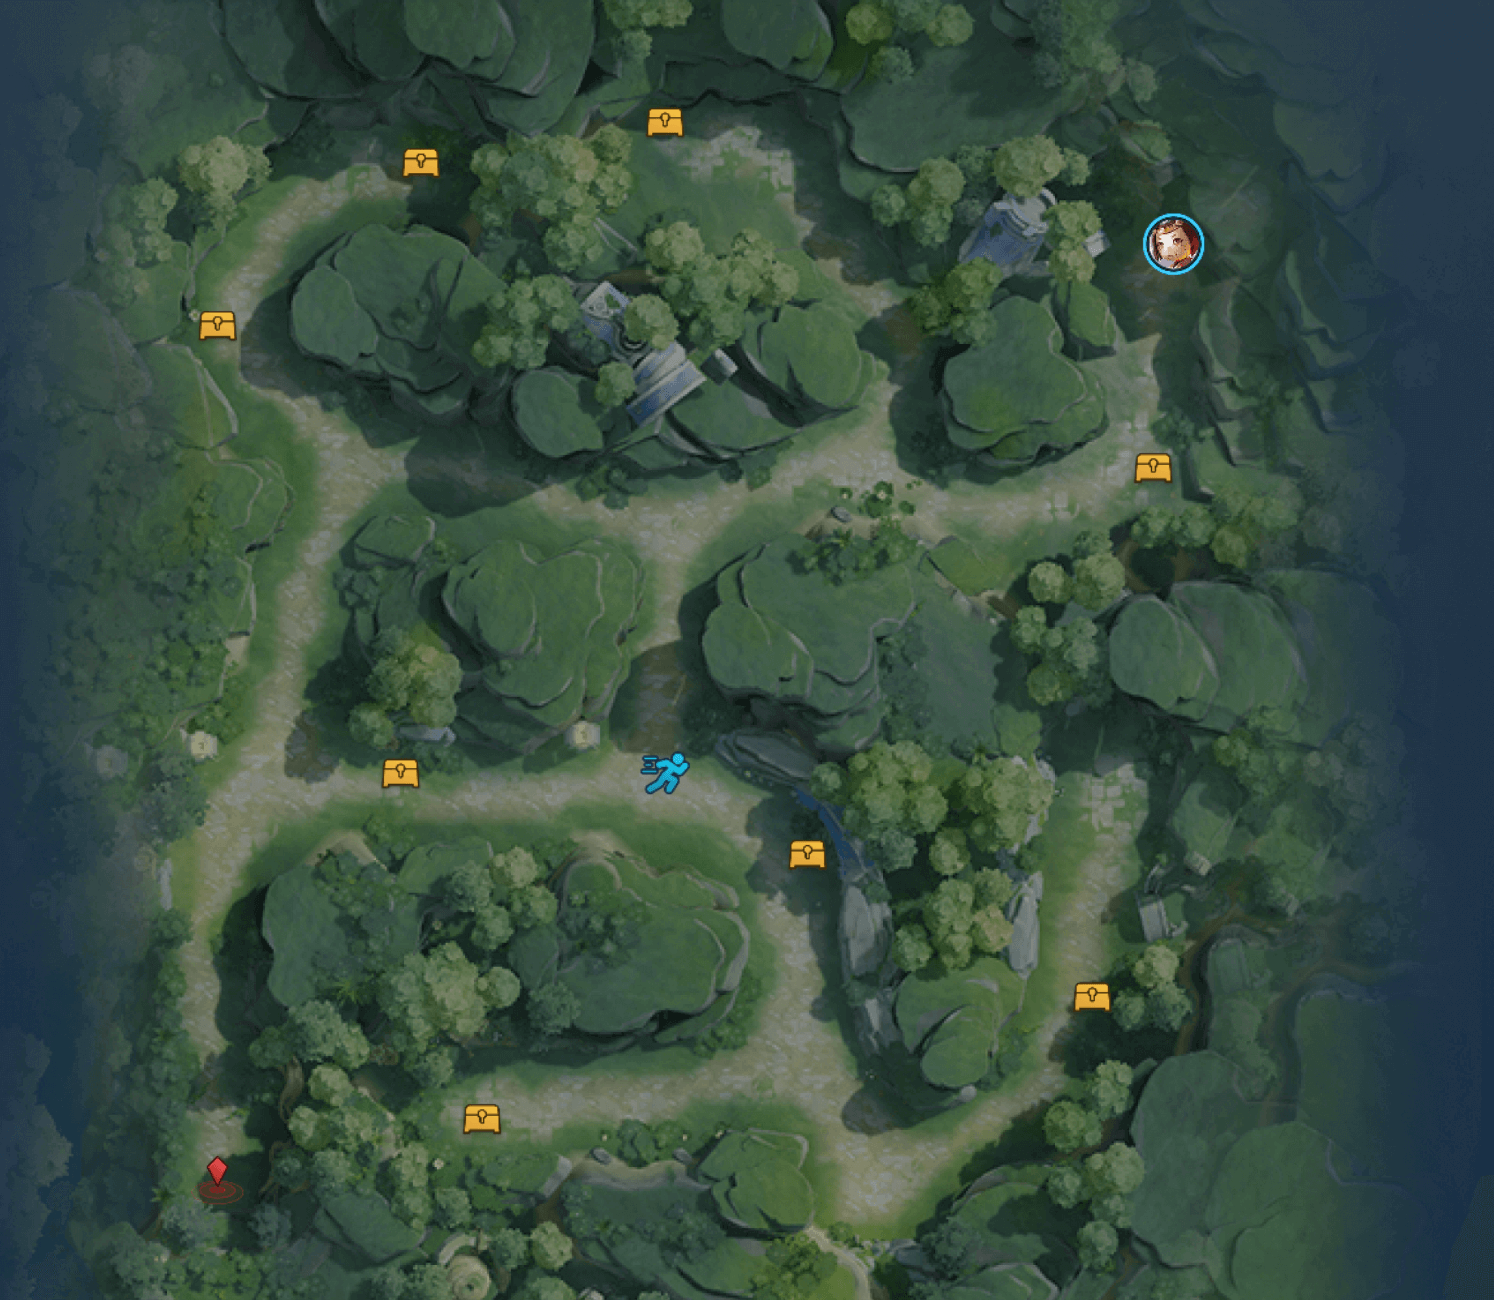
\includegraphics[width=0.8\linewidth]{pic/map.png}
    \caption{\zihao{-5} Map}
    \label{map}
\end{figure}

\Cref{elements} 中列举了地图中的所有元素。

\begin{table}[H]
    \begin{tabularx}{1\textwidth}{ l X } % | 表示垂直边框
        \hline % 水平边框
        \textbf{元素} & \textbf{说明}  \\
        \hline
        起点 & 任务开始时,智能体在起点出现。 \\
        终点 & 智能体的目的地,当智能体抵达终点时,任务结束。 \\
        道路 & 智能体可以在道路中有8个移动方向,智能体在执行一个动作后,会朝该动作表示方向持续移动3帧(1个step),然后在原地等待下一次动作指令。\\
        障碍物& 障碍物会阻挡智能体前进,当智能体在移动过程中遇到障碍物时,将紧贴障碍物边缘移动。有关智能体移动的详细介绍,请查看智能体移动及技能执行逻辑。\\
        宝箱 & 如果用户给任务配置了宝箱,则智能体可以通过拾取宝箱增加积分,每个宝箱获得100积分,地图中共有13个可配置宝箱的点位。可以通过配置宝箱的 数量 和 随机性 来调整环境的复杂度。 \\
        加速增益 & 在重返秘境地图中心存在一个加速增益,智能体可以通过拾取加速增益来提升自身的移动速度。在拾取加速增益后,移动速度提升 40\%,持续 10秒(约50个Step)。在增益结束后,智能体恢复默认速度。加速增益被拾取后会在 90秒(约454个Step) 后重新出现。 \\
        \hline
    \end{tabularx}

    \centering
    \caption{地图元素}
    \label{elements}
\end{table}

\subsubsection{智能体介绍}

\begin{enumerate}
    \item 视野域

    在重返秘境环境中,智能体只有局部视野:以智能体所在位置为中心,分别向“上、下、左、右”四个方向拓宽 25 格数的一个正方形观察域(size=51x51)。

    \item 技能

    智能体有 超级闪现 技能,使用该技能可以使智能体向指定方向位移8000。技能冷却时间 120秒(约606个Step)。
    当智能体使用超级闪现时,如果闪现的目的地在障碍物内(不在可移动的道路范围内),本次闪现技能将使用失败。
\end{enumerate}

\subsubsection{计分规则}

每一次游戏用户可以设定最大步数,如果智能体在最大步数内(包括最大步数)成功抵达终点,则判定任务成功,并按下方规则计算任务得分:

任务得分 = 终点得分 + 步数得分 + 宝箱得分

\begin{enumerate}
    \item 终点得分:到达终点即获得150分。
    \item 步数得分:(最大步数 - 完成步数) * 奖励系数0.2,完成步数是智能体抵达终点所用的步数。
    \item 宝箱得分:每获得一个宝箱,即可增加100分。
\end{enumerate}

注意:若在最大步数内没有走到终点,则判定为任务超时。超时任务的得分为0。

\subsection{环境介绍}

用户可以在 算法名称/train\_workflow.py 的 workflow 函数的参数中获取重返秘境环境 env:

\begin{adjustbox}{width=0.8\textwidth, center}
\begin{lstlisting}[language=Python]
def workflow(envs, agents, logger=None, monitor=None):
    env = envs[0] 
\end{lstlisting}
\end{adjustbox}

\quad

环境env有两个接口: reset 和 step,用户可以简单地通过以下方式来调用重返秘境环境:

\quad

\begin{adjustbox}{width=0.8\textwidth, center}
\begin{lstlisting}[language=Python]
obs = env.reset(usr_conf=usr_conf)
frame_no, _obs, score, terminated, truncated, env_info = env.step(act)
\end{lstlisting}
\end{adjustbox}

\subsubsection{环境配置}

用户可以在reset时传入一个usr\_conf来实现定制化的环境配置。
usr\_conf是一个字典类型,需要先定义一个 key 叫做 diy,diy的值包含一些键值对:

\begin{table}[H]
    \begin{tabularx}{1\textwidth}{ l l X } % | 表示垂直边框
        \hline % 水平边框
        \textbf{数据名} & \textbf{数据类型} & \textbf{说明}  \\
        \hline
        start & int & 起点编号,范围是[1,15],起点和终点不能重复 \\
        end & int & 终点编号, 范围是[1,15],起点和终点不能重复 \\
        treasure\_random & int & 是否生成随机宝箱,设置为1表示随机宝箱,设置为0表示固定宝箱,其他值非法 \\
        treasure\_num & int & 生成随机宝箱时的宝箱数量,仅在treasure\_random=1时生效,范围是 [1, 13] \\
        treasure\_id & list & 生成固定宝箱时的宝箱编号,仅在treasure\_random=0时生效,范围是 [1, 15],需要排除起点和终点编号,如果需要固定生成0个宝箱则传入[ ] \\
        max\_step & int & 单局最大步数,默认值为2000,无特殊需求不建议设置,过大的值会导致训练缓慢 \\
        talent\_type & int & 智能体技能,默认值为1,其他值非法 \\
        \hline
    \end{tabularx}

    \centering
    \caption{环境配置}
    \label{user-conf}
\end{table}

每个位置id对应的位置如\Cref{position}所示:

\begin{figure}[H]
    \centering
    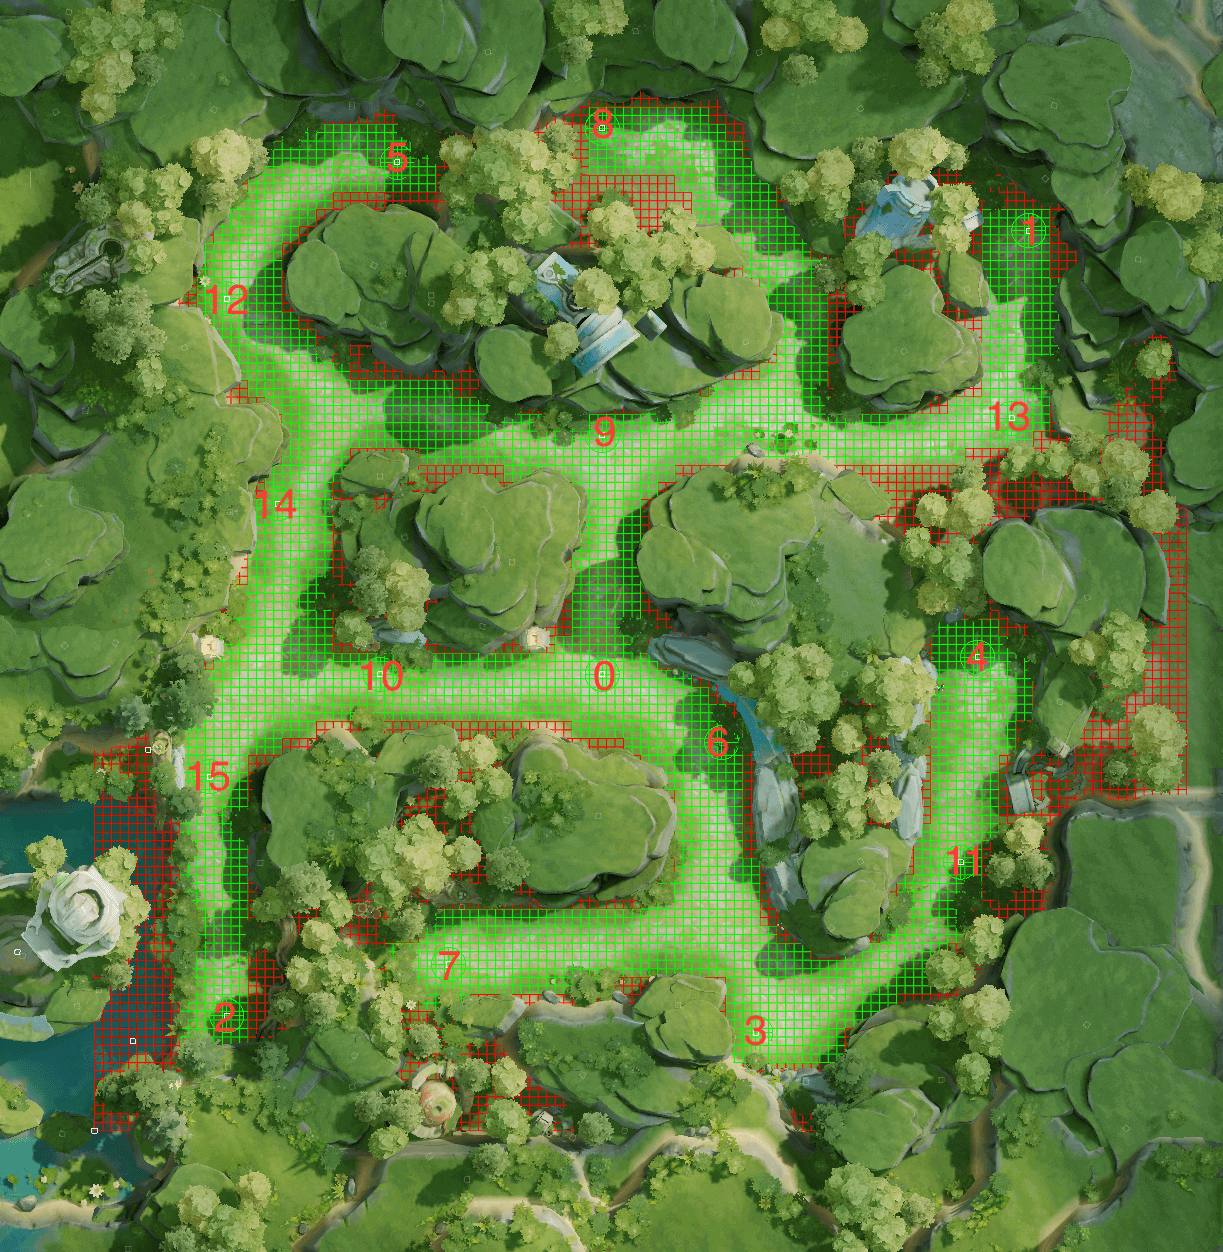
\includegraphics[width=0.8\linewidth]{pic/position.png}
    \caption{\zihao{-5} Position}
    \label{position}
\end{figure}

以下提供几个 usr\_conf 的设置实例:


\begin{enumerate}[label=例子\arabic*]
    \item 
\begin{lstlisting}[language=Python]
# 起点为2,终点为1,固定6个宝箱[4, 5, 6, 7, 8, 9]
usr_conf = {
    "diy": {
        "start": 2,
        "end": 1,
        "treasure_id": [4, 5, 6, 7, 8, 9],
        "treasure_random": 0,
        "talent_type": 1,
        "max_step": 2000,
    }
}
\end{lstlisting}

    \item 

\begin{lstlisting}[language=Python]
# 起点为2,终点为1,随机8个宝箱
usr_conf = {
  "diy": {
      "start": 2,
      "end": 1,
      "treasure_random": 1,
      "talent_type": 1,
      "treasure_num": 8,
      "max_step": 2000,
  }
}
\end{lstlisting}

    \item 

\begin{lstlisting}[language=Python]
# 起点为2,终点为1,固定0个宝箱
usr_conf = {
    "diy": {
        "start": 2,
        "end": 1,
        "treasure_id": [],
        "treasure_random": 0,
        "talent_type": 1,
        "max_step": 2000,
    }
}
\end{lstlisting}

\end{enumerate}

\subsection{环境信息}

用户调用env.step可以返回环境下一时刻的所有状态,以下 \Cref{environment-data} 是这些数据的描述,具体可以参考数据协议。


\begin{table}[H]
    \begin{tabularx}{1\textwidth}{l l X } % | 表示垂直边框
        \hline % 水平边框
        \textbf{数据名} & \textbf{数据类型} & \textbf{数据描述}  \\
        \hline
        frame\_no & int32 & 当前帧数 \\
        obs & <class 'custom\_pb2.Observation'> & 环境状态信息(观测信息) \\
        score & <class 'custom\_pb2.ScoreInfo'> & 得分信息 \\
        terminated & int32 & 表示游戏结束,即走到终点 \\
        truncated & int32 & 表示任务中断(超时或异常) \\
        env\_info & <class 'custom\_pb2.EnvInfo'> & 其他环境信息 \\
        \hline
    \end{tabularx}

    \centering
    \caption{环境数据}
    \label{environment-data}
\end{table}

用户调用env.reset可以返回环境的第一帧的状态,但仅包含观测空间obs。

\subsubsection{观测空间}

\Cref{measure-space} 返回的观测信息包含了当前环境的状态信息,具体包含属性feature和legal\_act,以下是这些数据的描述:

\begin{table}[H]
    \begin{tabularx}{1\textwidth}{l l X } % | 表示垂直边框
        \hline % 水平边框
        \textbf{数据名} & \textbf{数据类型} & \textbf{数据描述}  \\
        \hline
        norm\_pos&FloatPosition&归一化后的绝对坐标\\
        grid\_pos&Position&网格坐标\\
        start\_pos&RelativePosition&起点的相对位置\\
        end\_pos&RelativePosition&终点的相对位置\\
        buff\_pos&list(RelativePosition)&加速增益的相对位置\\
        treasure\_pos&RelativePosition&宝箱的相对位置\\
        obstacle\_map&list&周边障碍物信息\\
        memory\_map&list&周边记忆地图信息\\
        treasure\_map&list&周边宝箱信息\\
        end\_map&list&周边终点信息\\
        legal\_act&list&环境当前状态的可执行的动作        \\
        \hline
    \end{tabularx}

    \centering
    \caption{观测空间}
    \label{measure-space}
\end{table}

\subsubsection{位置信息}

以norm\_pos和grid\_pos为例,分别表示归一化后的绝对坐标和网格坐标,分别为FloatPosition类型和Position类型,norm\_pos由grid\_pos计算得到

\begin{lstlisting}[language=Python]
# FloatPosition的协议描述
message FloatPosition {
    float x = 1;                // x坐标
    float z = 2;                // z坐标
}
# Position的协议描述
message Position {
    int32 x = 1;                // x坐标
    int32 z = 2;                // z坐标
}
# 示例代码
pos = Position(x=100, z=100)
float_pos = FloatPosition(
        x=pos.x/64000,
        z=pos.z/64000,
)
\end{lstlisting}

\subsubsection{相对位置信息}

下面是对 \Cref{rel-pos} RelativePosition 详细的描述:

\begin{enumerate}
\item RelativePosition 表征的是英雄在任意位置时,物件的相对位置信息,比如方向,距离。其中:
\item RelativeDirection 通过枚举离散化表示方向信息。

RELATIVE\_DIRECTION\_NONE East NorthEast North NorthWest West SouthWest South SouthEast

\item RelativeDistance 通过枚举离散化表示距离信息。

RELATIVE\_DISTANCE\_NONE VerySmall Small Medium Large VeryLarge

\item path\_distance和grid\_distance是通过将地图网格化后计算出的从英雄当前格子到目标格子的网格路径最短距离,前者进行了离散化处理,后者进行了归一化处理。
\end{enumerate}


\begin{table}[H]
    \begin{tabularx}{1\textwidth}{l l X } % | 表示垂直边框
        \hline % 水平边框
        \textbf{RelativePosition} & \textbf{数据类型} & \textbf{数据描述}  \\
        \hline
        direction&RelativeDirection&相对方位(离散化)\\
        l2\_distance&RelativeDistance&L2距离(离散化)\\
        path\_distance&RelativeDistance&网格化后的最短路径距离(离散化)\\
        grid\_distance&float&网格化后的最短路径距离(归一化)        \\
        \hline
    \end{tabularx}

    \centering
    \caption{RelativePosition}
    \label{rel-pos}
\end{table}


\subsubsection{观测视野范围}

智能体观测到的地图范围是有限的,我们在观测空间中提供了智能体的视野域信息,即英雄周围的网格化后的局部信息。如 \Cref{scope} 所示:

\begin{figure}[H]
    \centering
    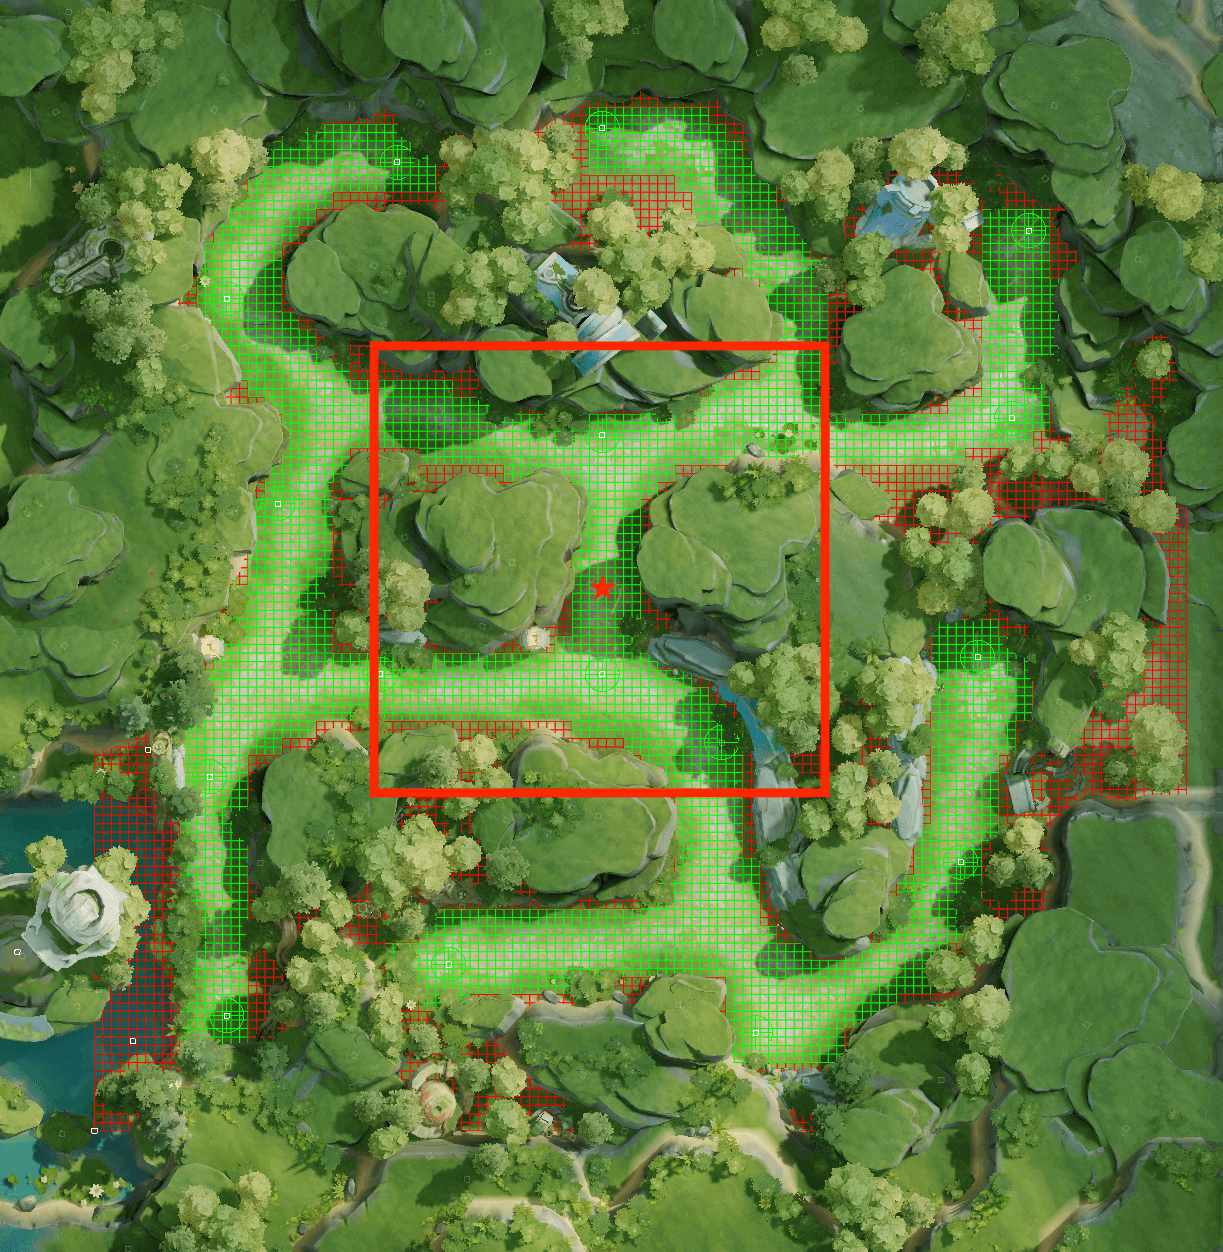
\includegraphics[width=0.8\linewidth]{pic/scope.png}
    \caption{\zihao{-5} 视野范围}
    \label{scope}
\end{figure}

\Cref{visible-scope} 视野域中会标注出障碍物、宝箱、终点以及记忆信息,分别存储在obstacle\_map、treasure\_map、end\_map、memory\_map四个向量中。


\begin{table}[H]
    \begin{tabularx}{1\textwidth}{l  X } % | 表示垂直边框
        \hline % 水平边框
        \textbf{向量名} & \textbf{说明}  \\
        \hline
        obstacle\_map&向量长度为2601,是51x51的矩阵视野域的一维展开,有阻挡的位置为0,无阻挡的位置为1。\\
        memory\_map&记录智能体探索每一个网格区域的次数,归一化到[0,1],初始化为0,每抵达一个网格,该网格坐标对应的值+0.2,最大为1。\\
        treasure\_map&标注宝箱的位置,有宝箱的位置为1,否则为0。\\
        end\_map&标注终点的位置,有终点的位置为1,否则为0。\\
        \hline
    \end{tabularx}

    \centering
    \caption{视野域}
    \label{visible-scope}
\end{table}

\subsection{动作空间}

重返秘境的动作空间分为两个部分:移动和技能,总的Action维度为16。env.step()传入的参数取值范围是[0, 15]


\subsubsection{移动}

移动使用的是8维离散化的动作空间,如\Cref{action-space}所示,将360度等分为8份,每45度角一个动作方向,以x轴正方向为起点,逆时针旋转。

\begin{figure}[H]
    \centering
    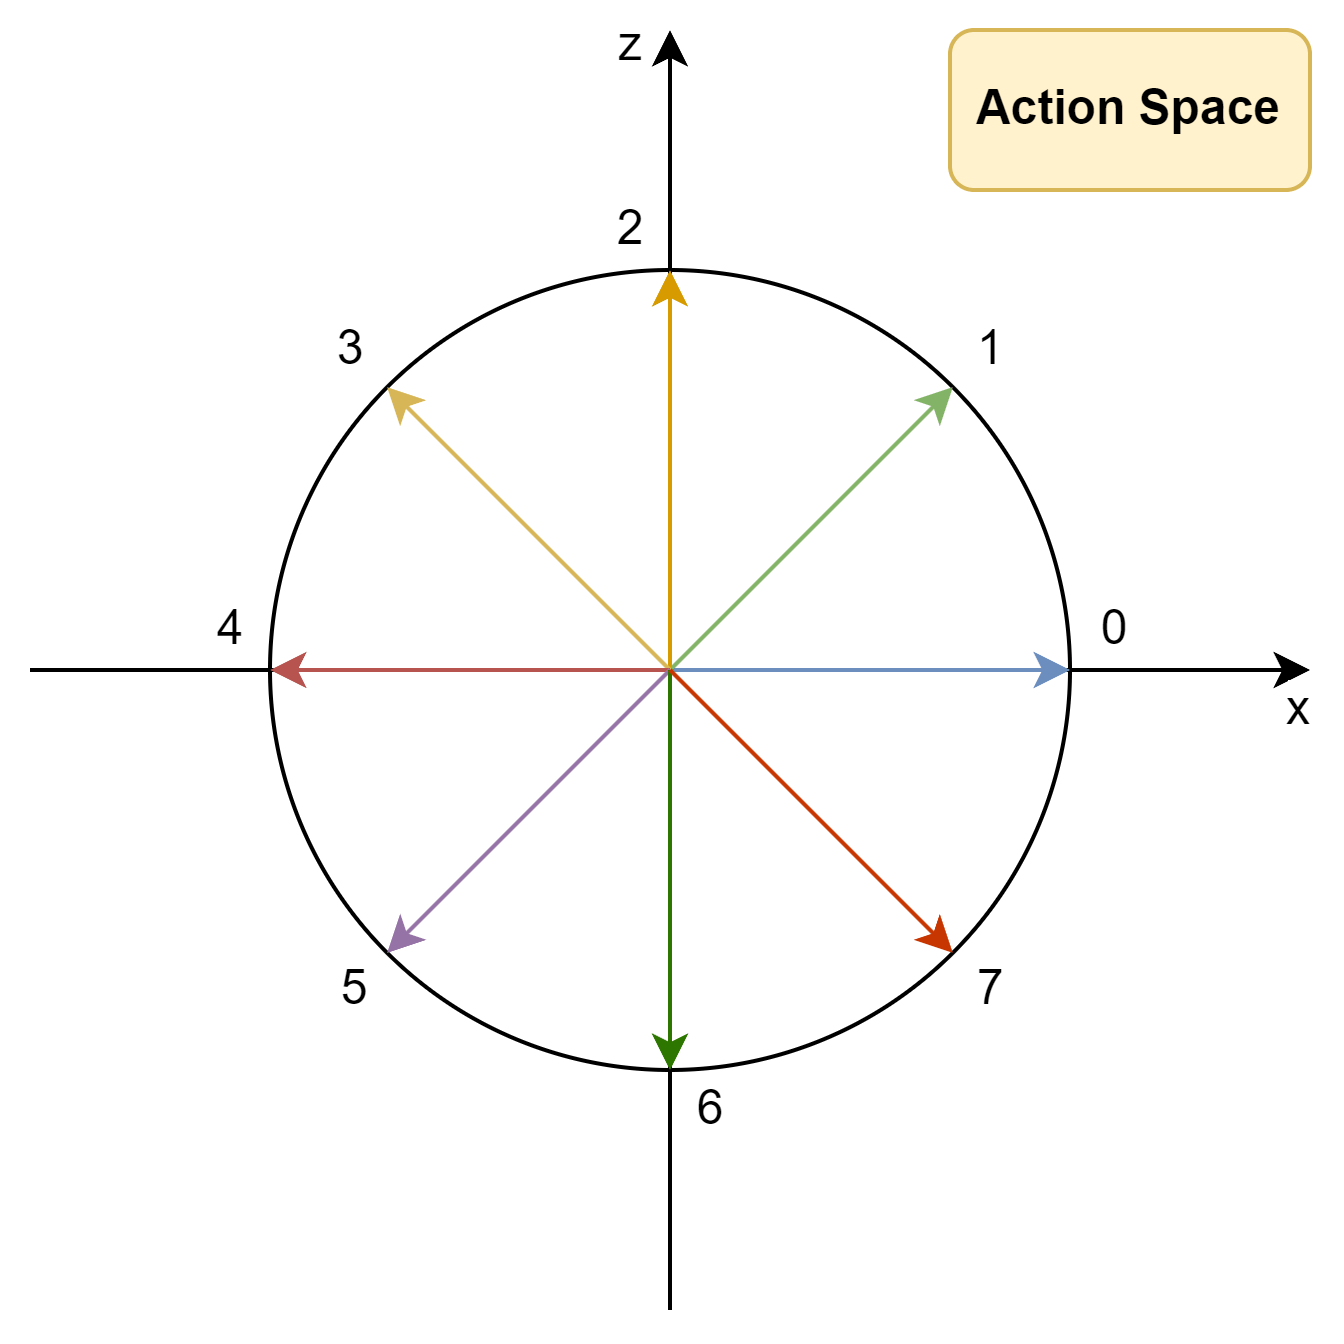
\includegraphics[width=0.8\linewidth]{pic/action-space.png}
    \caption{\zihao{-5} 移动}
    \label{action-space}
\end{figure}

对应关系如下:

\begin{lstlisting}[language=Python]
// 方向角,以x轴正方向为起始边
enum Direction {
    Angle_0 = 0;
    Angle_45 = 1;
    Angle_90 = 2;
    Angle_135 = 3;
    Angle_180 = 4;
    Angle_225 = 5;
    Angle_270 = 6;
    Angle_315 = 7;
}
\end{lstlisting}

我们将移动用一个8维的one-hot vector来表征,比如Direction = Angle\_90时,Action[0:8] = [0, 0, 1, 0, 0, 0, 0, 0]

\subsubsection{技能}

智能体有 超级闪现 技能,技能默认CD为120秒,闪现距离为8000,超级闪现的方向和移动方向一致。技能同样也是用一个8维的one-hot vector来表征,比如使用超级闪现且超级闪现方向Direction = Angle\_270时,Action[8:16] = [0, 0, 0, 0, 0, 0, 1, 0]。

\subsubsection{执行逻辑}


接下来介绍智能体移动和技能的执行逻辑。如\Cref{move}所示,在一次决策中,首先必须给智能体提供一个方向(8维的Direction),然后:

\begin{enumerate}
    \item  如果智能体执行移动动作,那么智能体会沿着该方向移动,一次预测(3帧)的移动距离大概为700,加速状态为1000。
    \begin{enumerate}
\item 移动方向上无障碍物:正常移动。
\item 移动方向上有障碍物:如下图白色箭头,移动方向的命令为Angle\_45=1, 实际执行时由于障碍物的阻挡,会沿着下方的白色箭头贴着障碍物的边缘移动。
    \end{enumerate}

    \item 如果智能体执行超级闪现动作,那么智能体会沿着该方向闪现,闪现距离为8000。

    \begin{enumerate}
\item 闪现方向上无障碍物:正常闪现,如下图的红色例子。
\item 闪现方向上有障碍物:
\item 闪现的目标位置无障碍物:穿墙闪现,如下图的蓝色箭头。
\item 闪现的目标位置有障碍物:闪现失败,原地不动,如下图的黄色箭头,英雄还是处于方块位置不动
    \end{enumerate}
\end{enumerate}


\begin{figure}[H]
    \centering
    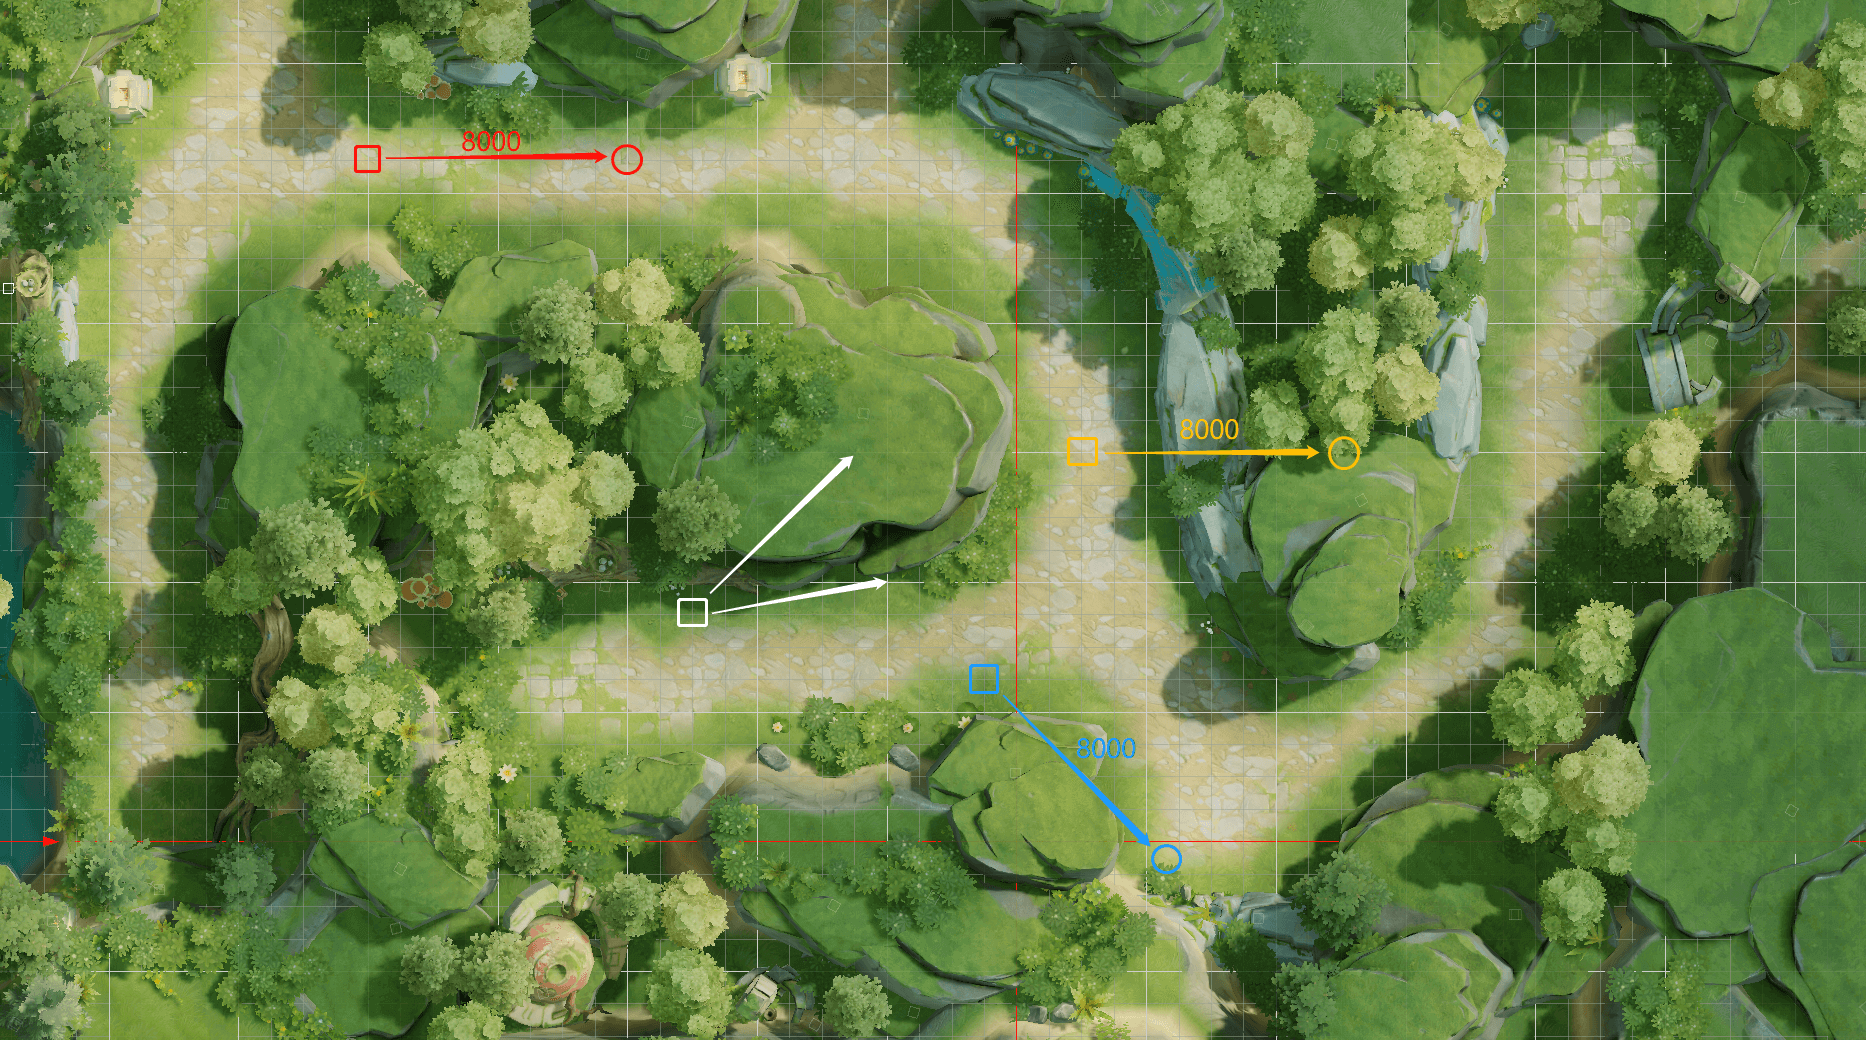
\includegraphics[width=0.8\linewidth]{pic/move.png}
    \caption{\zihao{-5} 移动}
    \label{move}
\end{figure}

补充说明:

\subsubsection{合法动作}

在环境中的某一时刻,不是所有的动作都可以被执行,因此我们需要向模型输入legal action,将网络结果进行掩码(masking)从而避免不符合规则的动作被输出。

在重返秘境中,超级闪现作为一个可执行的动作在冷却未结束时需要被避免使用,因此,在我们默认设置里将超级闪现是否可使用的信息作为legal action输入。

在默认设置里,legal\_action的输入为二维,第一维代表移动方向,第二维代表超级闪现方向。在超级闪现可以使用的时候移动和超级闪现都被允许预测,因此我们返还 [1, 1], 在超级闪现冷却时超级闪现不被允许输出,因此我们返还[1, 0]。在DQN算法的网络中输出16维的Q值信息,前八维对应八个可行走方向,后八维对应八个可超级闪现方向,第一维legal\_action对应前八维输出,第二维legal\_action对应后八维输出。

\subsection{得分信息}

env.step(act) 返回的 score 是在当前状态下执行动作 act 智能体所获得的分数,分数的计算详见计分规则。

\subsection{时间信息}

帧(frame)和步(step)存在一定映射关系。

帧是场景的一个时间单位,表示场景的一个完整更新周期。在每一帧中,场景的所有元素(如宝箱等)都会根据当前的状态和输入进行更新。

步是强化学习环境中的一个时间单位,表示智能体(agent)在环境中执行一个动作并接收反馈的过程。在每一步中,智能体选择一个动作,环境根据该动作更新状态,并返回新的状态、奖励和终止信号。

在本环境中,1个step由3个frame组成。这意味着每个动作对应一个步,在每一步中,智能体将在三个连续的帧中执行同一个动作。环境将在每一步结束后更新状态并返回反馈,场景只有在完成三帧后,环境状态才会返回一次状态的更新。

\begin{enumerate}
\item 步更新:在每一步中,智能体选择一个动作,环境更新状态并返回。
\item 帧更新:在一步中,场景进行三次帧更新,更新所有场景中对象的状态并渲染新的画面。
\end{enumerate}

帧(frame),步(step),现实时间秒(s)和现实时间毫秒(ms)的关系如下:

\begin{align*}
    1\,\text{frame} = 60 \,\text{ms} \\
    1\,\text{step} = 3\,\text{frame} \\
    1\,\text{s} = 1000\,\text{ms} \\
\end{align*}


注意 :由于运行环境的差异,每一帧的时间会在66毫秒上下浮动

\subsection{监控介绍}

在腾讯开悟平台的训练管理页面,提供了查看监控功能,点击后,即可在新标签页中打开监控面板,如下图所示。可以通过查看监控数据实时定位自己的训练进程,从而帮助大家评更快更准确的找到问题所在。

\subsubsection{监控面板介绍}

在监控面板中,包括 错误日志数量 和 监控指标图 两部分内容。

错误日志数量:在该模块中,可以看到训练过程中每个模块的错误日志数量。点击模块卡片可以进入日志详情页,查看该模块的错误日志信息。

监控指标图:在该模块中,可以看到四类数据指标,分别是basic(基础指标)、algorithm(算法指标)、env(环境指标)、diy(自定义指标)。

\begin{table}[H]
    \begin{tabularx}{1\textwidth}{ l X } % | 表示垂直边框
        \hline % 水平边框
        \textbf{指标分类} & \textbf{说明}  \\
        \hline
        basic&包括强化学习训练过程中的标准数据和资源使用数据。\\
        algorithm&和算法相关的数据指标,不同算法上报的指标可能会有所不同。\\
        env&和环境相关的数据指标,不同环境上报的指标不同。\\
        diy&用户自行上报的数据指标。\\
        \hline
    \end{tabularx}

    \centering
    \caption{监控面板}
    \label{monitor-dashboard}
\end{table}


\begin{enumerate}
    \item 基础指标

\begin{table}[H]
    \begin{tabularx}{1\textwidth}{ l X } % | 表示垂直边框
        \hline % 水平边框
        \textbf{指标名称} & \textbf{说明}  \\
        \hline
    train\_global\_step&训练的累计步数,即agent.learn的调用次数。取决于各算法的具体实现:DQN系列的算法从样本池中采样一次后调用agent.learn。\\
    predict\_succ\_cnt&采样预测的累计帧数,即agent.predict的调用次数。\\
    sample\_production\_and\_consumption\_ratio&等于训练步数除以采样预测的累计帧数。\\
    episode\_cnt&已经结束的任务个数。\\
    load\_model\_succ\_cnt&预测加载模型文件成功的次数,即调用agent.load\_model的调用次数。\\
    sample\_receive\_cnt&learner成功接收的样本数量。\\
        \hline
    \end{tabularx}
    \centering
    \caption{基础指标}
    \label{monitor-basic}
\end{table}


    \item 算法指标

\begin{table}[H]
    \begin{tabularx}{1\textwidth}{ l X } % | 表示垂直边框
        \hline % 水平边框
        \textbf{指标名称} & \textbf{说明}  \\
        \hline
        reward&累积回报,反应了智能体的能力,正常训练情况下指标应该是震荡向上。\\
        q\_value&target网络的Q值,一定程度反应Q值的稳定性。\\
        value\_loss&计算loss的标量值,反应训练的进程,正常情况下指标应该是逐渐接近于0。\\
        \hline
    \end{tabularx}
    \centering
    \caption{算法指标}
    \label{monitor-alg}
\end{table}

    \item 环境指标

\begin{table}[H]
    \begin{tabularx}{1\textwidth}{ l X } % | 表示垂直边框
        \hline % 水平边框
        \textbf{指标名称} & \textbf{说明}  \\
        \hline
        score & 该面板包含两个指标:total\_score:任务结束时的得分,若任务超时,则该局得分为0。treasure\_score:任务结束时收集到的宝箱奖励。\\
        steps & 该面板包含两个指标:max\_steps:任务设置的最大步数。finished\_steps:任务结束时所用的步数。若任务超时,则该局完成步数等于最大步数。\\
        treasure & 该面板包含两个指标:total\_treasures:任务设置的宝箱个数。collected\_treasures:任务结束时收集到的宝箱个数。\\
        treasure\_random & 宝箱是否随机。若为0则表示宝箱位置固定,若为1则表示宝箱位置随机。\\
        skill\_cnt & 技能使用次数。\\
        buff\_cnt & 加速增益拾取次数。\\
        \hline
    \end{tabularx}
    \centering
    \caption{环境指标}
    \label{monitor-env}
\end{table}

    \item diy(自定义指标)

    我们提供了五个自定义指标diy\_1至diy\_5以便用户可以上报自己想要监控的数据。

    \begin{figure}[H]
        \centering
        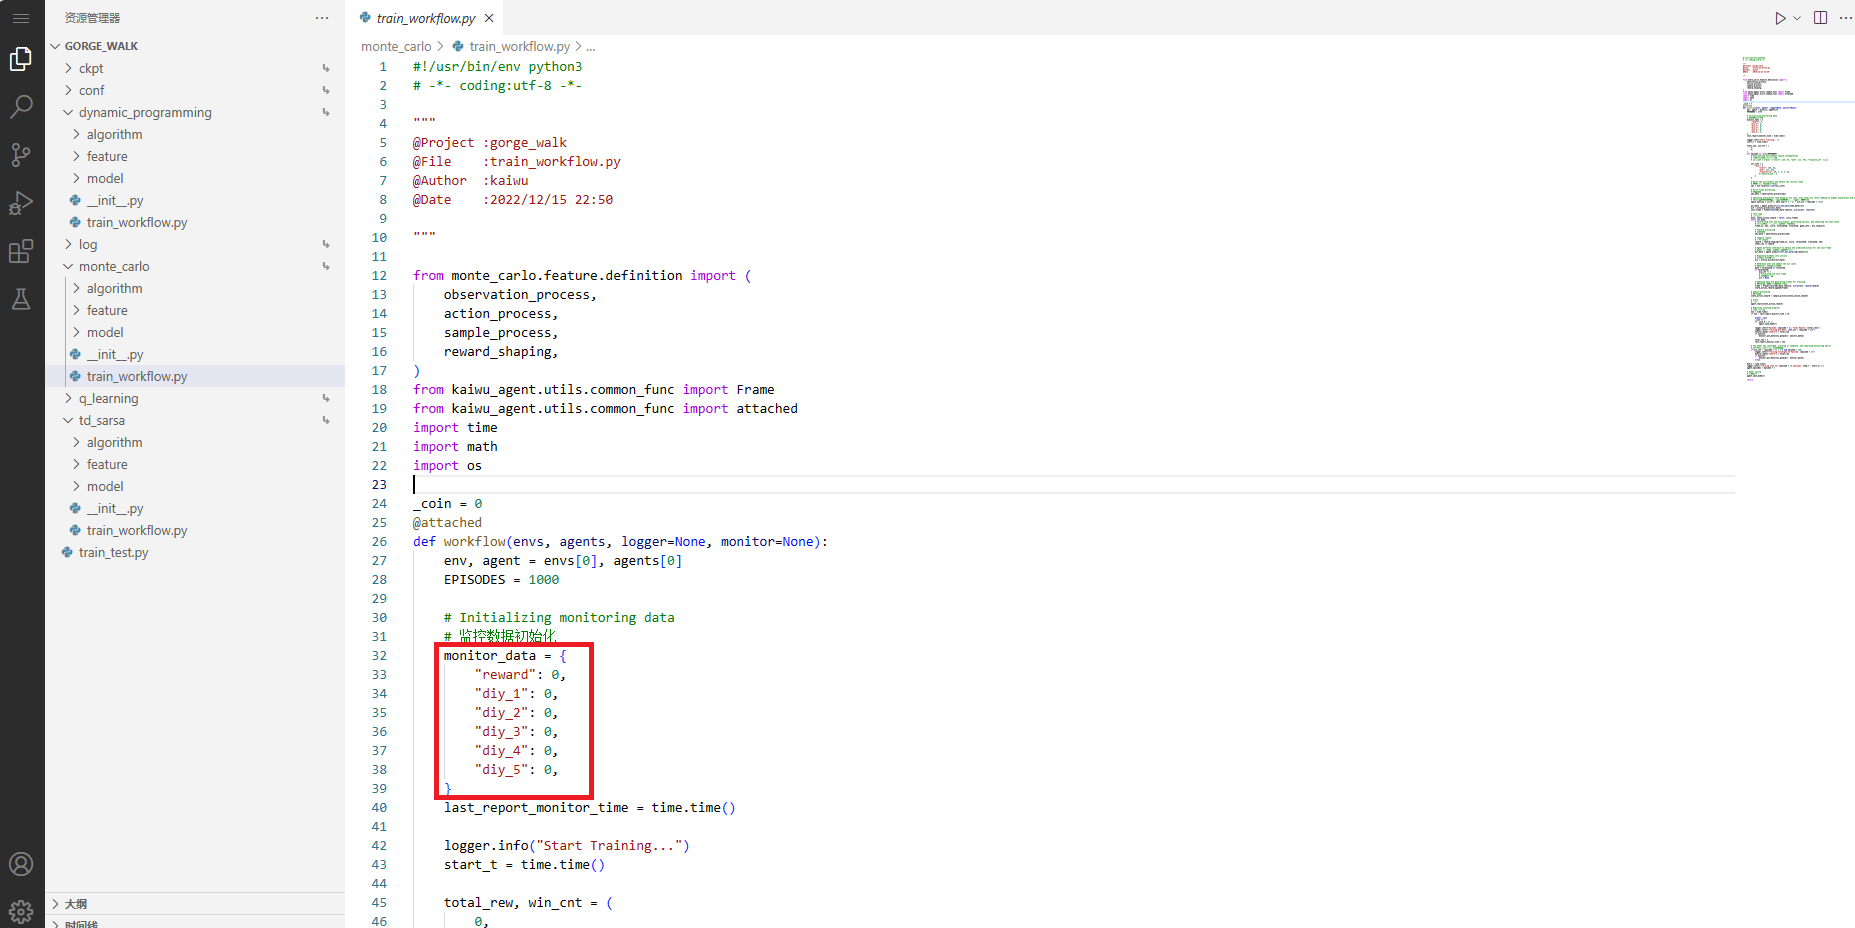
\includegraphics[width=1\linewidth]{pic/diy.png}
        \caption{\zihao{-5} 自定义指标}
        \label{diy}
    \end{figure}

\end{enumerate}


\section{实验准备}

\subsection{代码包介绍}

\subsubsection{目录介绍}


\begin{table}[H]
    \begin{tabularx}{1\textwidth}{ l X } % | 表示垂直边框
        \hline % 水平边框
        \textbf{目录名} & \textbf{介绍}  \\
        \hline
        dqn&dqn 算法子目录\\
        target\_dqn&target\_dqn 算法子目录\\
        diy&Do it yourself 用户自定义算法的子目录\\
        conf&配置文件\\
        train\_test.py&代码正确性测试脚本\\
        \hline
    \end{tabularx}

    \centering
    \caption{代码目录}
    \label{directory}
\end{table}

其中 dqn,target\_dqn 是重返秘境场景的 2 个核心算法,diy为用户自定义的算法。各个算法的子目录结构如下:

\begin{table}[H]
    \begin{tabularx}{1\textwidth}{ l X } % | 表示垂直边框
        \hline % 水平边框
        \textbf{目录名/文件名} & \textbf{介绍}  \\
        \hline
        algorithm/&算法相关,主要是 agent 的实现,包含训练和预测,详情见算法开发\\
        feature/&特征相关,主要包含用户自定义的数据结构和数据处理方法,以及特征和奖励的计算,详情见实现特征处理和样本处理\\
        model/&模型相关,主要是模型的实现,是一个Model类\\
        config.py&该算法下的配置,用户可以任意增加配置或修改配置,注意:SAMPLE\_DIM是开悟框架使用配置,不允许删除\\
        train\_workflow.py&强化学习的训练流程,详情见强化学习训练流程开发        \\
        \hline
    \end{tabularx}

    \centering
    \caption{自定义算法}
    \label{directory:alg}
\end{table}


\subsection{开发流程}

概括来说,我们的开发任务是:开发智能体和智能体的训练流程,这个智能体包含一个可被训练的模型,智能体可以对环境给出的观测进行决策,这个决策作用于环境产生新的观测,此过程通过训练流程控制,不断循环。训练流程还要收集循环过程中产生的每一帧数据,将他们组合成样本数据,智能体可以根据这些样本作为算法的输入,通过算法更新模型。由于重返秘境采用分布式训练,会启动多个容器,样本需要通过网络通信发送到训练容器(learner)中进行训练,所以需要对样本进行编码方便网络发送,另外智能体需要将learner容器上的模型同步回来。以上任务可以描述为 \Cref{dev-process}:

\begin{figure}[H]
    \centering
    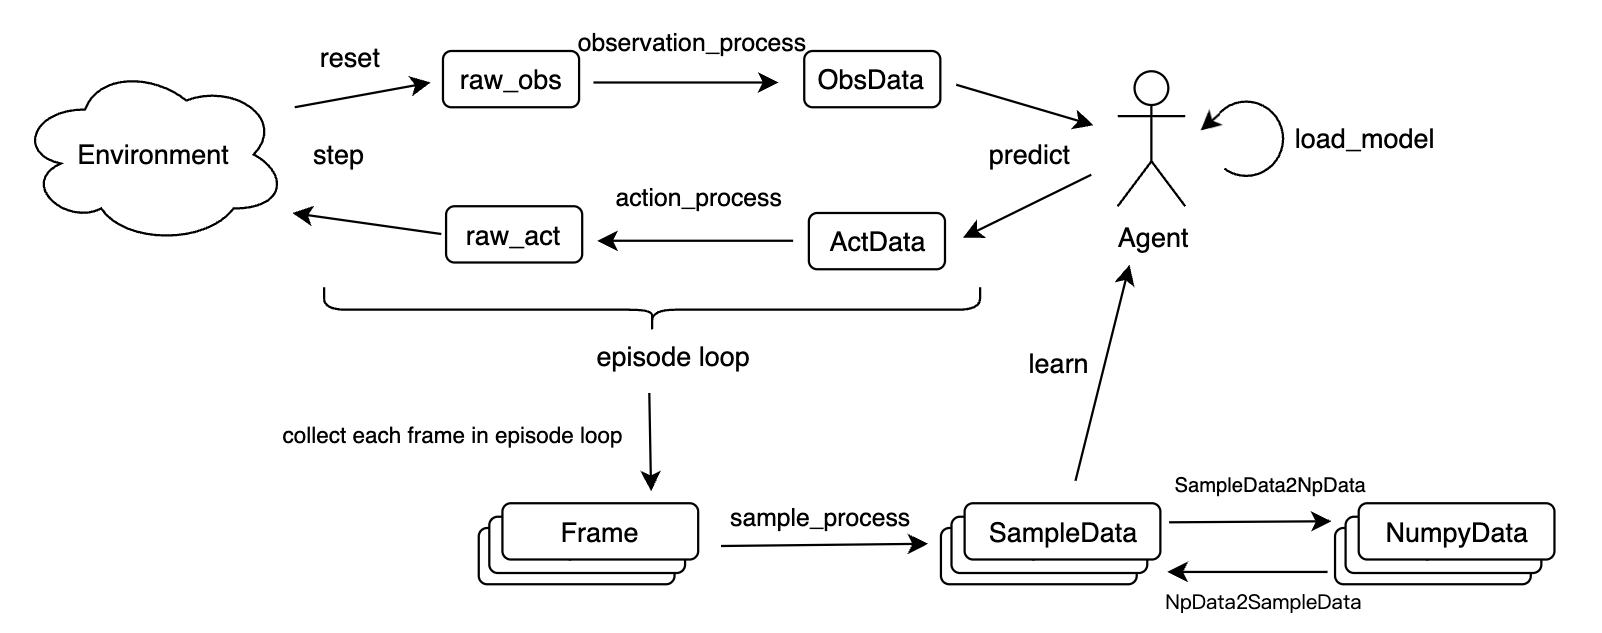
\includegraphics[width=1\linewidth]{pic/dev-process.png}
    \caption{\zihao{-5} 开发流程}
    \label{dev-process}
\end{figure}

开发流程如下:

\begin{enumerate}
\item 定义数据结构:一般情况下,环境产生的原始观测数据不能直接作为智能体的输入,并且不同的用户开发的智能体一般是不一样的,显然不同的智能体的决策、学习方法的输入输出也是不一样的,所以开发的第一步,我们应该定义智能体输入输出的数据结构。包括特征(ObsData)、动作(ActData)、样本(SampleData),其中ObsData和ActData分别作为智能体predict方法的输入和输出,SampleData作为智能体learn方法的输入。
\item 实现特征处理和样本处理:不同的用户实现不同的智能体可能会定义不同的数据结构,但是,环境接口输入输出的数据结构是固定的,因此环境接口的输入输出数据和智能体接口的输入输出数据需要进行转换,所以还需要用户实现这些数据结构的转换方法,包括:observation\_process, action\_process, sample\_process。
\item 算法开发:用户需要实现一个 agent,agent中实现一个模型(一般是神经网络模型)。agent负责与环境交互,产生预测动作并训练模型。
\item 实现强化学习训练流程:在实现了 数据结构,数据处理函数,模型和 智能体 以及其他方法(如奖励处理函数)后,我们还需要实现一个强化学习的训练流程workflow,将所有组件组合起来完成强化学习训练,即智能体通过不断的与环境交互,获取样本数据,更新并迭代模型,直到模型收敛到我们想要的效果。
\item 训练参数配置:在分布式训练时,开悟平台会启动一个样本池,一个模型同步服务,这些组件的相关参数用户可以根据自己的设计进行配置
\end{enumerate}


\begin{figure}[H]
    \centering
    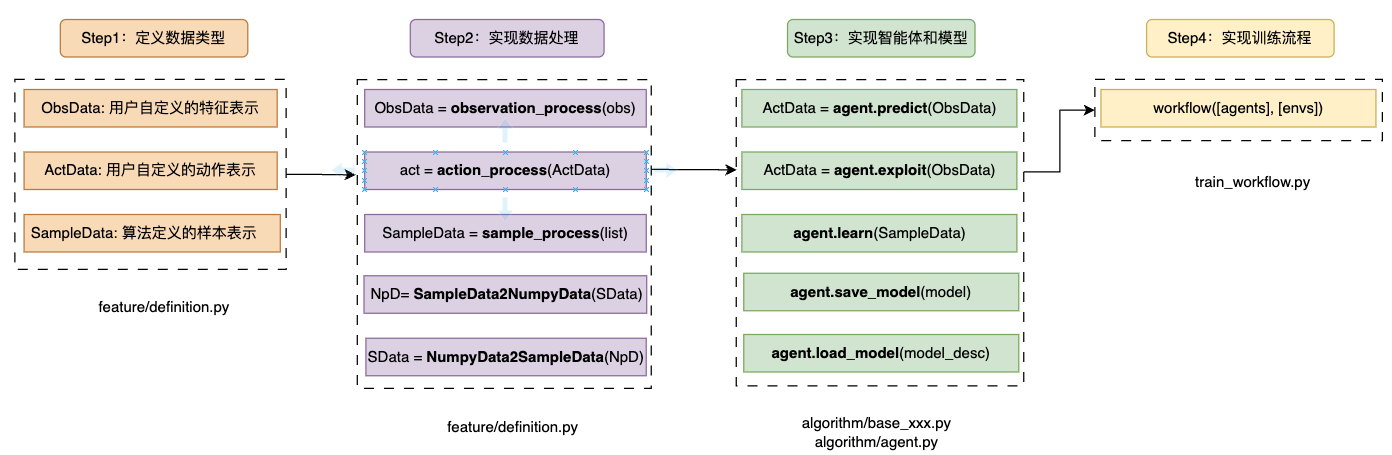
\includegraphics[width=1\linewidth]{pic/dev-process-1.png}
    \caption{\zihao{-5} 开发流程}
    \label{dev-process-1}
\end{figure}

分布式训练架构如 \Cref{train} 所示,

\begin{figure}[H]
    \centering
    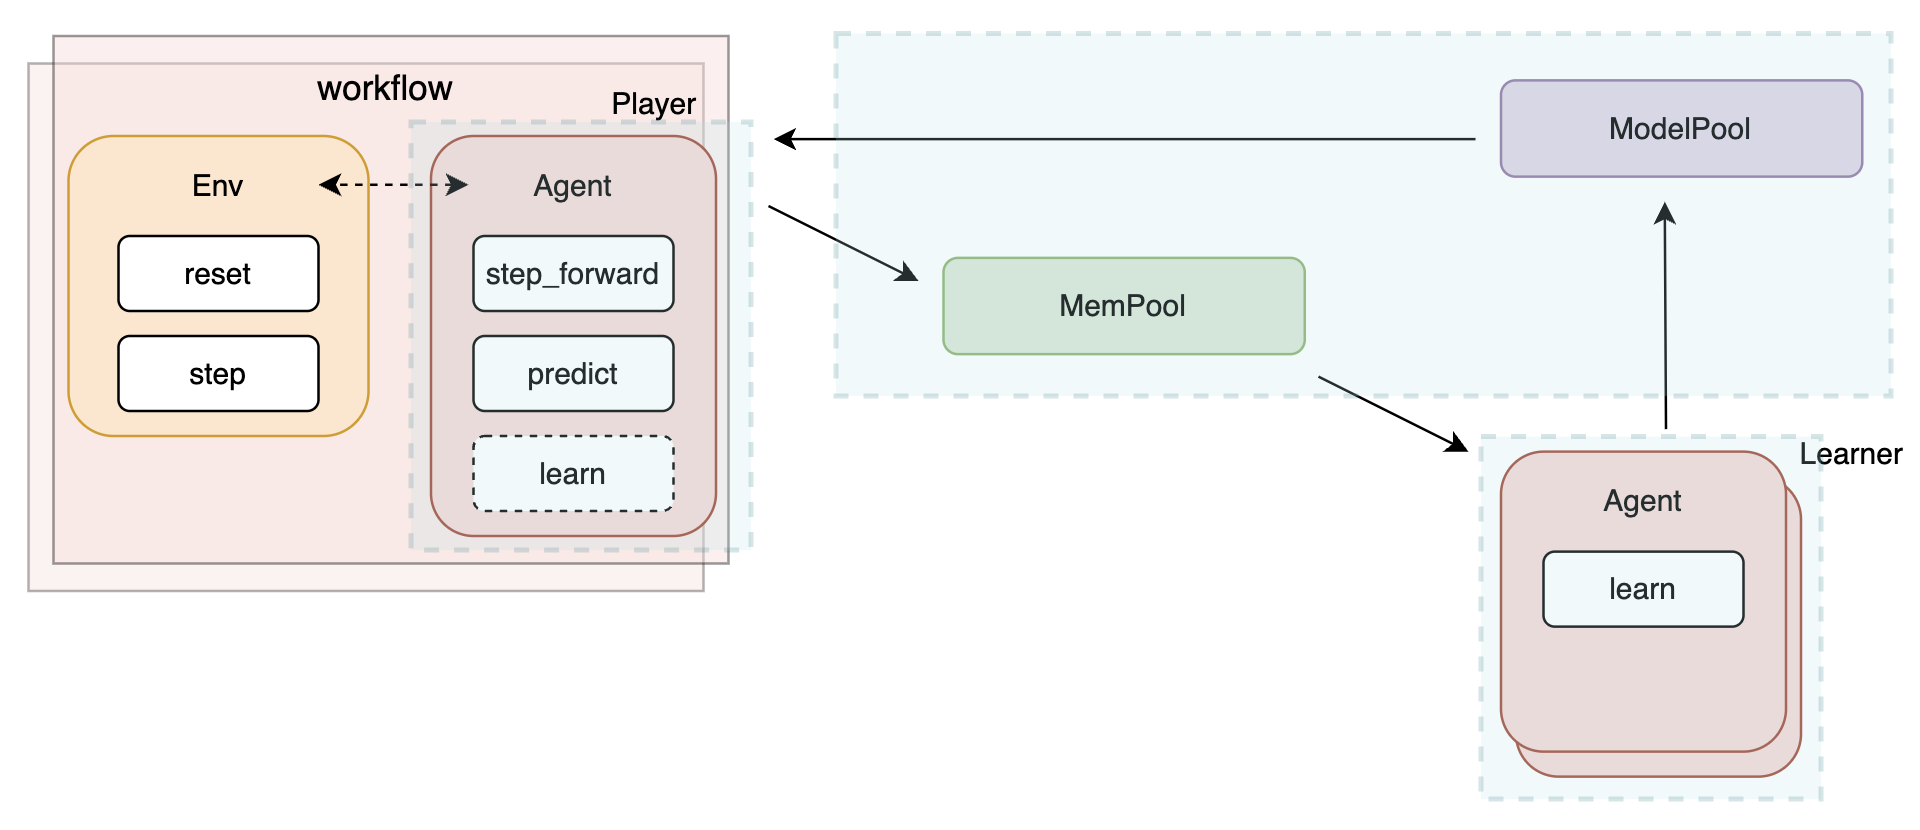
\includegraphics[width=1\linewidth]{pic/train.png}
    \caption{\zihao{-5} 分布式训练架构}
    \label{train}
\end{figure}

特别注意: 因为重返秘境会进行分布式训练,开悟平台会启动一个样本池(样本先进先出),用户的agent.learn(samples)调用将会把样本发送到样本池,训练容器会从样本池中采样样本samples将其传入agent.learn(samples)进行训练,此过程是自动的,用户无需开发额外代码.

\subsubsection{定义数据结构}

环境介绍里详细描述了环境返回的原始观测信息 obs,这里的 obs 已经做了一定的数据预处理工作,但是智能体是由用户设计和实现的,环境使用的obs, act等与智能体的输入输出是存在差异的,所以要先定义数据结构(类)再进行数据转换,包括:包括特征(ObsData)、动作(ActData)、样本(SampleData),这部分的代码,都需要实现在<算法名称>/feature/definition.py中。

我们以 DQN 算法为例,介绍解决环境配置为固定宝箱时的数据类型定义。

首先需要定义相关的数据结构(类)包含观测数据ObsData,动作数据ActData,和样本数据SampleData, 其中ObsData和ActData分别表示智能体预测的输入和输出,将会由agent.predict使用;SampleData为样本的数据类型,样本数据将会被agent.learn中的代码进行处理用于模型的训练。这些数据结构(类)包含哪些属性完全由用户自定义,属性名称属性数量没有限制。

create\_cls函数用于动态创建一个类,create\_cls的第一个参数为类型名称,剩余参数为类的属性,属性默认值为None。以下是代码示例:

\begin{lstlisting}[language=Python]
# The create_cls function is used to dynamically create a class. The first parameter of the function is the type name,
# and the remaining parameters are the attributes of the class, which should have a default value of None.
# create_cls函数用于动态创建一个类,函数第一个参数为类型名称,剩余参数为类的属性,属性默认值应设为None
ObsData = create_cls("ObsData",
    feature=None,
    legal_act=None)

ActData = create_cls("ActData",
    move_dir=None,
    use_talent=None)

SampleData = create_cls("SampleData",
    obs=None,
    _obs=None,
    obs_legal=None,
    _obs_legal=None,
    act=None,
    rew=None,
    ret=None,
    done=None) 
\end{lstlisting}

\subsubsection{实现特征处理和样本处理}

用户需要实现特征处理,动作处理,样本处理,和奖励设计函数,例如环境返回的数据属于原始观测数据,是无法直接作为智能体预测时的输入的,我们需要实现特征处理函数(observation\_process),将环境返回的原始观测数据转换成用户定义的ObsData。这部分的代码,都需要实现在<算法名称>/feature/definition.py中。

我们依然以 DQN算法为例,介绍解决环境配置为固定宝箱时的特征处理和样本处理。

需要实现特征处理和样本处理的函数有:observation\_process, action\_process, sample\_process。


\begin{table}[H]
    \begin{tabularx}{1\textwidth}{ X X X X } % | 表示垂直边框
        \hline % 水平边框
        \textbf{函数名} & \textbf{输入} & \textbf{输出} & \textbf{描述} \\
        \hline
        observation\_process&env.reset和env.step返回的原始观测数据raw\_obs&用户定义的ObsData类型的数据&将环境返回的原始观测数据转换成用户定义的ObsData类型数据\\
        action\_process&用户定义的ActData类型的数据&env.step能处理的动作数据&将智能体预测返回的ActData类的数据转换成env.step能处理的动作数据\\
        sample\_process&在环境中收集的每一帧信息组成的列表&SampleData类型的数据组成的列表&将环境数据帧的集合转换为样本的集合\\
        \hline
    \end{tabularx}

    \centering
    \caption{函数描述}
    \label{functions}
\end{table}

\subsubsection{奖励设计}

这里的奖励特指强化学习中的Reward,注意要与项目简介中的计分规则区别开。任务得分用于衡量玩家在任务中的表现,也作为衡量强化学习训练后的模型的优劣。代码包里提供了一些奖励的实现,可以参考这部分代码<算法名称>/feature/definition.py里的reward\_shaping函数修改各个奖励的权重。
不仅可以设置权重,还可以在<算法名称>/feature/definition.py里的reward\_shaping函数去实现自己的reward设计。

\subsubsection{算法开发}

重返秘境目前支持以下算法:DQN,Target-DQN,另外,我们还留了一个未实现的算法DIY,提供给用户进行自定义算法的实现,以上每个算法的开发流程都是一致的,所以这里以 DQN 的代码为例,讲解 DQN 是如何实现的:

首先,如果我们需要实现一个神经网络模型,我们需要在文件<算法名称>/model/model.py中实现一个Model类,即用pytorch实现一个神经网络模型。

然后,我们需要在文件<算法名称>/algorithm/agent.py中实现一个 Agent类。注意Agent类需要继承 kaiwu\_agent.agent.base\_agent 的 BaseAgent 类,Agent类的实现需要符合BaseAgent类的接口规范

注意:Agent类必须使用@attached装饰器,代码默认已实现,注意不要删除。


\begin{lstlisting}[language=Python]
    class BaseAgent:
    """
    Agent 的基类,所有的 Agent 都应该继承自这个类"""
    def __init__(self, agent_type="player", device=None, logger=None, monitor=None) -> None:
        raise NotImplementedError

    def learn(self, list_sample_data) -> dict:
        """
        用于学习的函数,接受一个 SampleData 的列表
        """
        raise NotImplementedError

    def predict(self, list_obs_data: list) -> list:
        """
        用于获取动作的函数,接受一个 ObsData 的列表, 返回一个动作列表
        """
        raise NotImplementedError

    def exploit(self, list_obs_data: list) -> list:
        """
        用于获取动作的函数,接受一个 ObsData 的列表, 返回一个动作列表
        """
        raise NotImplementedError

    def save_model(self, path, id='1'):
        raise NotImplementedError

    def load_model(self, path, id='1'):
        raise NotImplementedError
\end{lstlisting}

Agent类有三个核心的方法predict,exploit,和learn,其中predict和exploit方法负责进行预测,区别在于前者是智能体训练时调用的方法,一般是依策略的概率分布采样或引入随机概率,后者是智能体在评估时调用的方法,一般是选取策略中概率最高的动作或者策略认为最优的动作;learn方法中实现了核心算法,主要负责消费样本进行模型训练,其示例代码如下:

\begin{lstlisting}[language=Python]
"""
DQN/algorithm/agent.py
"""
@attached
class Agent(base_dqn.Agent):
    def __init__(self, agent_type="player", device="cpu", logger=None, monitor=None):
        # 进行若干初始化操作
        # ...

    @predict_wrapper
    def predict(self, list_obs_data):
        return self.__predict_detail(list_obs_data, exploit_flag=False)

    @exploit_wrapper
    def exploit(self, list_obs_data):
        return self.__predict_detail(list_obs_data, exploit_flag=True)

    @learn_wrapper
    def learn(self, list_sample_data):
        # 算法详细代码不在此处展示
\end{lstlisting}


\subsubsection{强化学习流程}

在实现了 数据结构,数据处理函数,模型和 智能体 以及其他方法(如奖励处理函数)后,我们还需要实现一个强化学习的训练流程workflow将所有组件结合起来完成强化学习训练,即智能体通过不断的与环境交互,获取样本数据,更新并迭代模型,直到模型收敛。

完成了上述组件之后,需要再实现一个强化学习的训练流程workflow,来让智能体 Agent 和环境 Environment 不断的交互从而产生。


\begin{figure}[H]
    \centering
    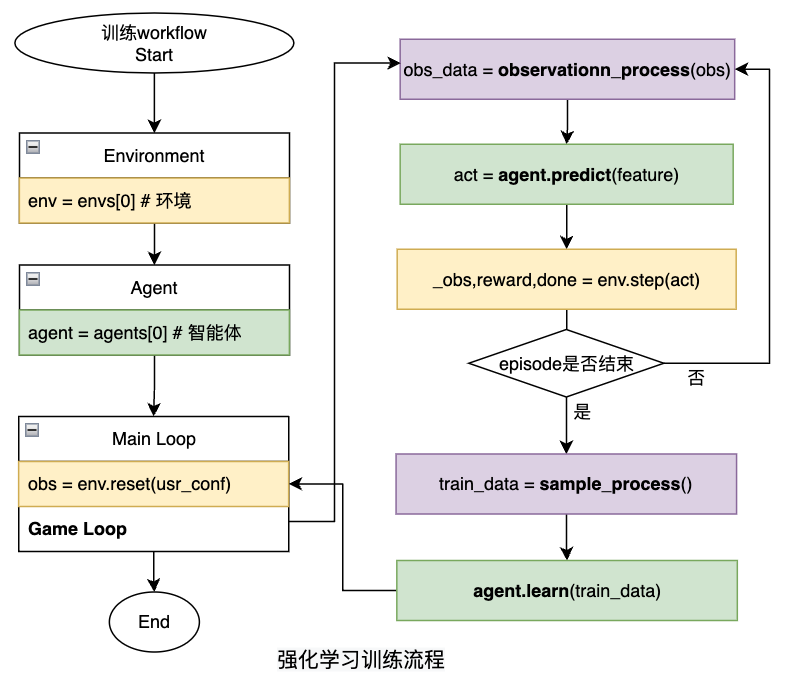
\includegraphics[width=0.8\linewidth]{pic/reinforcement.png}
    \caption{\zihao{-5} 强化学习流程}
    \label{reinforcement}
\end{figure}

\section{实验步骤}

\subsection{模型保存}

代码包中提供的workflow示例代码会保存模型,你也可以在workflow代码中的任意时机调用agent.save\_model保存中间模型。 注意:虽然agent.save\_model接受path和id两个参数,但在分布式训练时,workflow中调用该接口传入的参数会被框架覆盖成实际的模型保存路径以及最新的训练步数。

为了避免用户保存模型的频率过于频繁,模型保存会有安全限制,限制规则如下:

\begin{enumerate}
    \item 保存模型的频率限制: 2次/分钟
    \item
    单个任务保存模型的次数限制:(不同算法的限制不同)
    DQN or Target-DQN:100次
    DIY:100次
\end{enumerate}

\subsection{评估模式}

开悟平台支持评估模式,帮助用户在训练后评估模型的能力。相比较训练时用户可以在每一局设置usr\_conf,评估时用户需要在提交任务界面进行宝箱配置。另外,训练模式时,用户一般使用agent.predict方法进行决策;而在评估模式时,平台会调用agent.exploit方法进行决策,一般情况下,模型在训练和评估时的决策会因算法不同和用户设计不同,而有不同的行为,这部分由用户定义和实现。


\subsection{代码调试}

在代码包的根目录,我们提供了代码测试脚本train\_test.py,该脚本将使用算法文件夹下train\_workflow.py中的workflow进行一次训练,当训练步数>0时判定本次代码测试通过。通过启动一次训练,脚本能够迅速验证流程中的各个环节是否正确进行,确保训练逻辑的准确性。

为避免训练模型时出现因代码问题导致的错误,我们建议你在正式训练前一定要对代码进行测试。操作如下:

\begin{enumerate}
    \item 将train\_test.py文件中algorithm\_name的值修改为需要测试的算法名,算法名需要是algorithm\_name\_list中的一个。
    
    \item 进入IDE工具栏的【运行与调试】工具,点击下图所示绿色箭头的 运行 按钮。启动后,IDE会开始对代码进行测试,并将运行结果输出到右侧面板下方的终端区域,以方便你进行观察和分析。
\end{enumerate}

\begin{figure}[H]
    \centering
    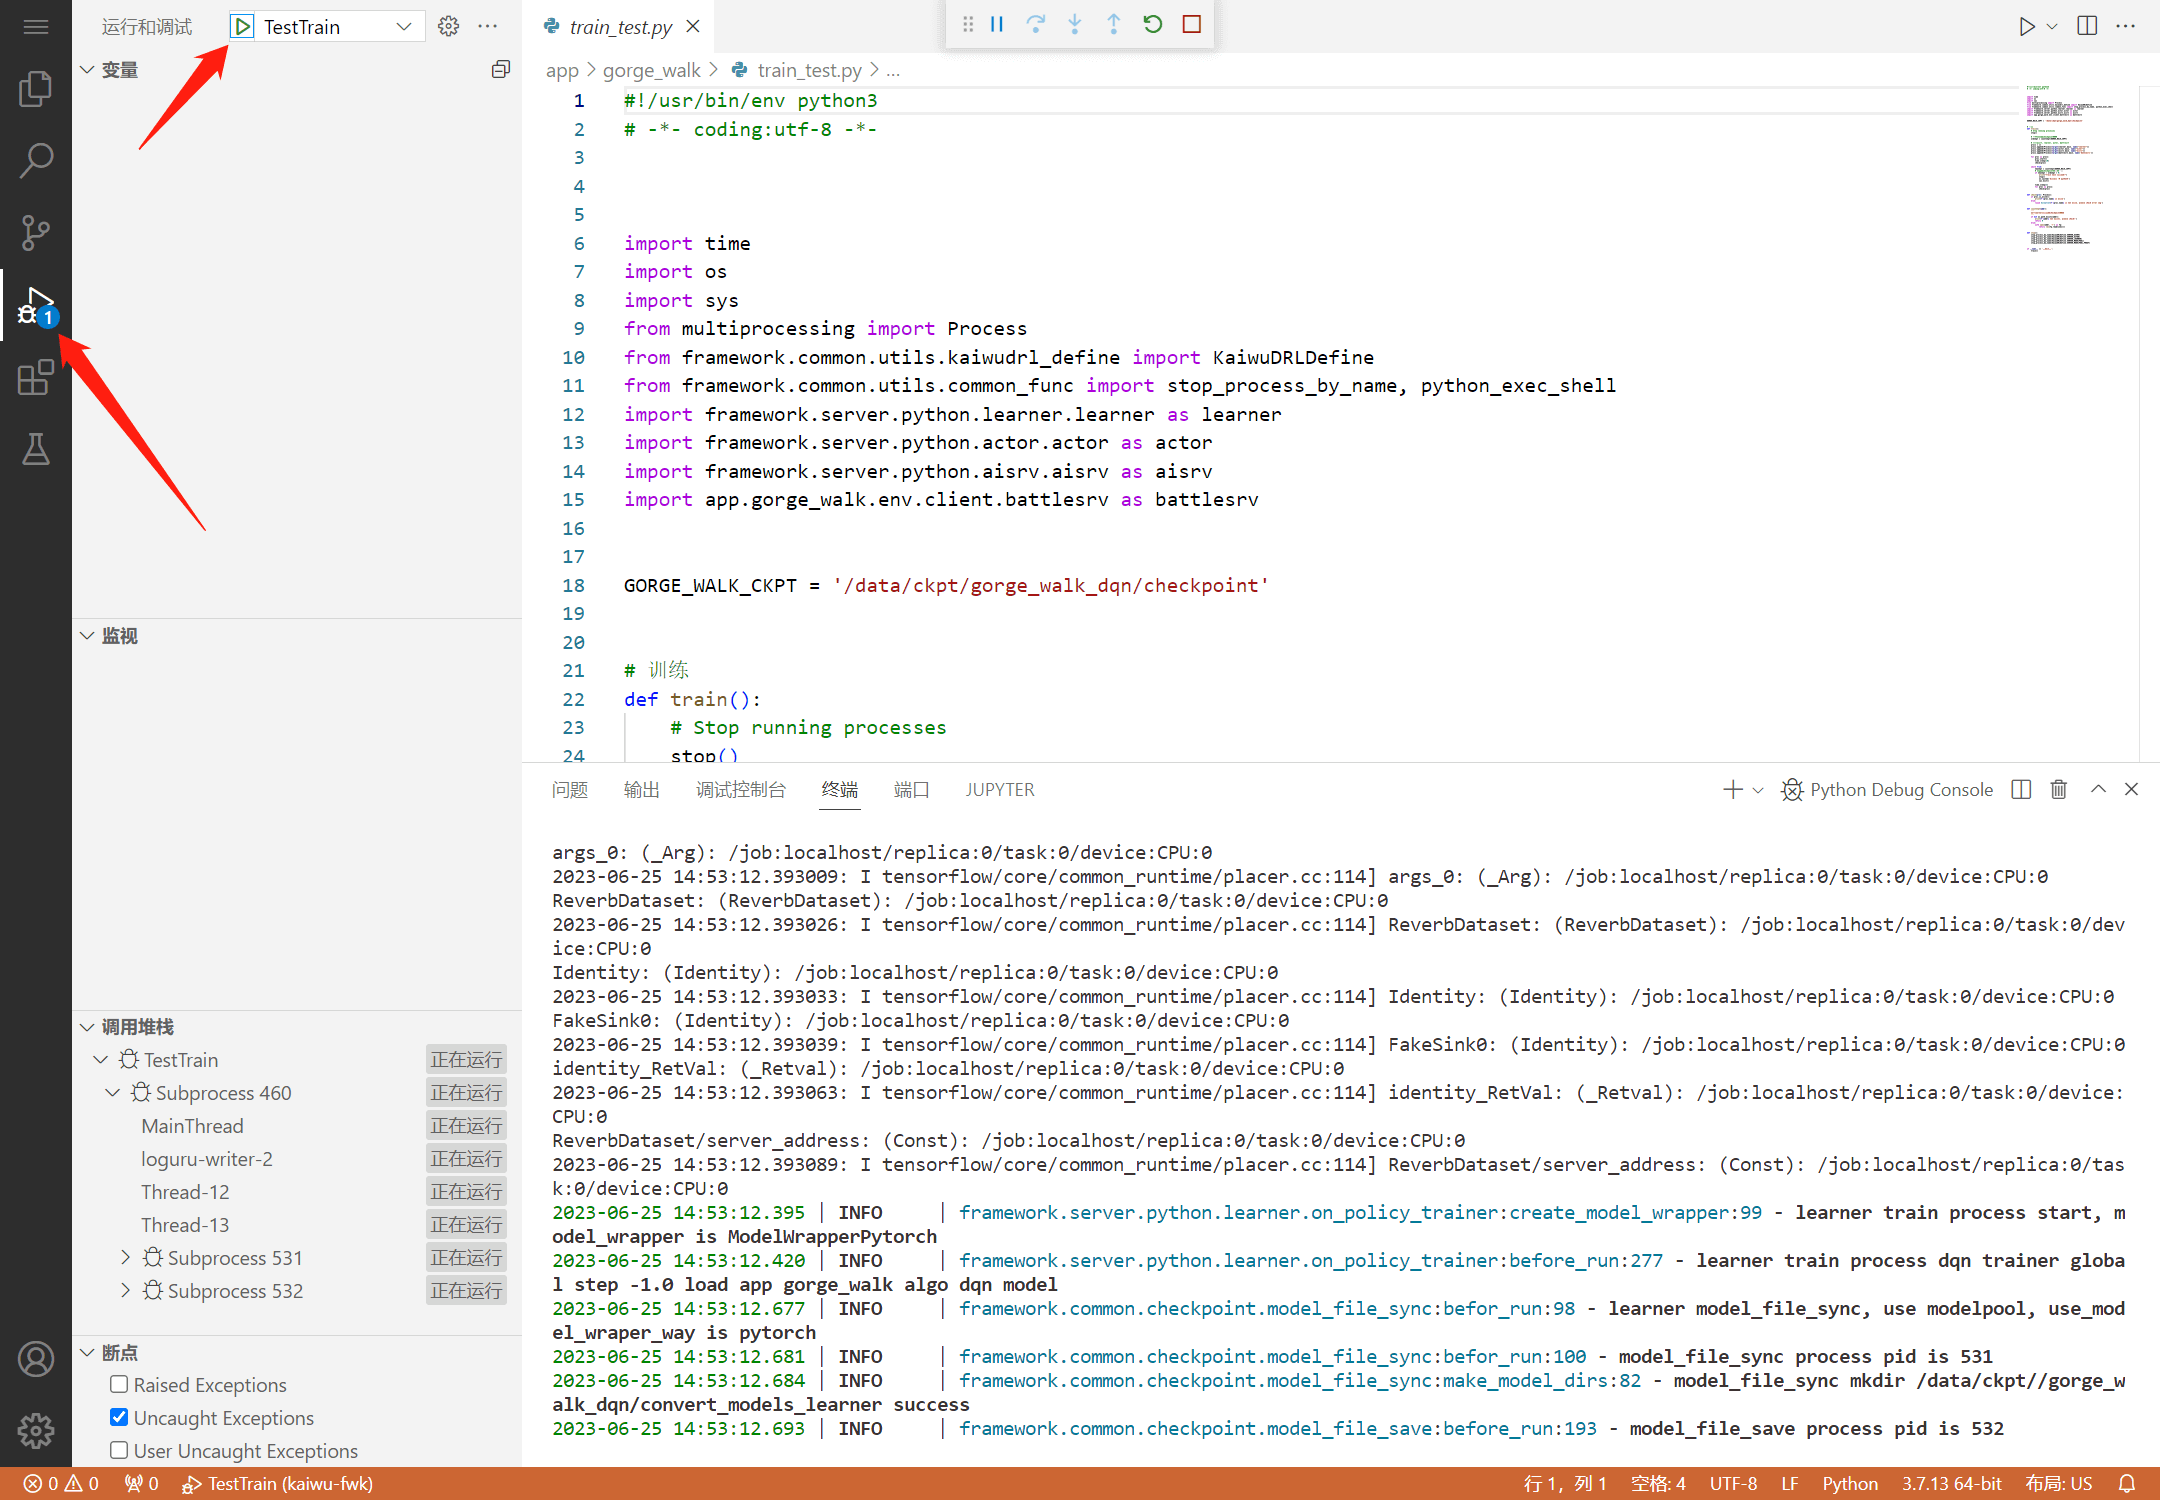
\includegraphics[width=1\linewidth]{pic/debug.png}
    \caption{\zihao{-5} 代码调试}
    \label{debug}
\end{figure}

在代码测试过程中如果遇到错误,则测试流程自动中止。此时你可以根据下方的终端面板查看错误信息,根据错误信息定位代码的问题。

如果没有遇到错误,则代码测试流程会在一次强化训练结束后自动终止(几分钟左右,请耐心等待),并在下方的终端面板提示Train test succeed。
\section{算法说明}

\subsection{DQN}
深度 Q 网络(Deep Q-Network,DQN)是一种基于深度学习和强化学习的算法,用于解决离散动作空间的强化学习问题。
\subsubsection{算法流程}
\begin{figure}[H]
    \centering
    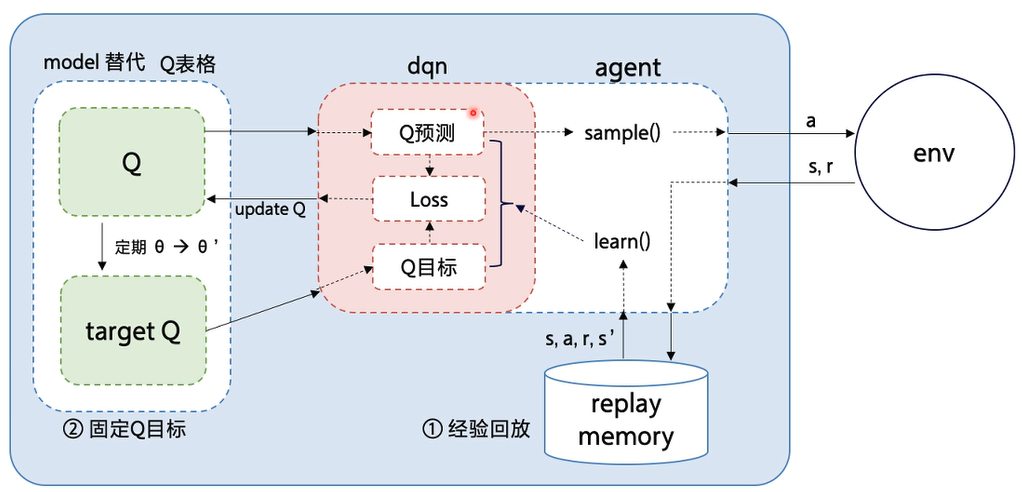
\includegraphics[width=0.8\linewidth]{pic/DQN-process.png}
    \caption{\zihao{-5} DQN算法流程}
    \label{map}
\end{figure}

\subsubsection{算法伪代码}
\begin{figure}[H]
    \centering
    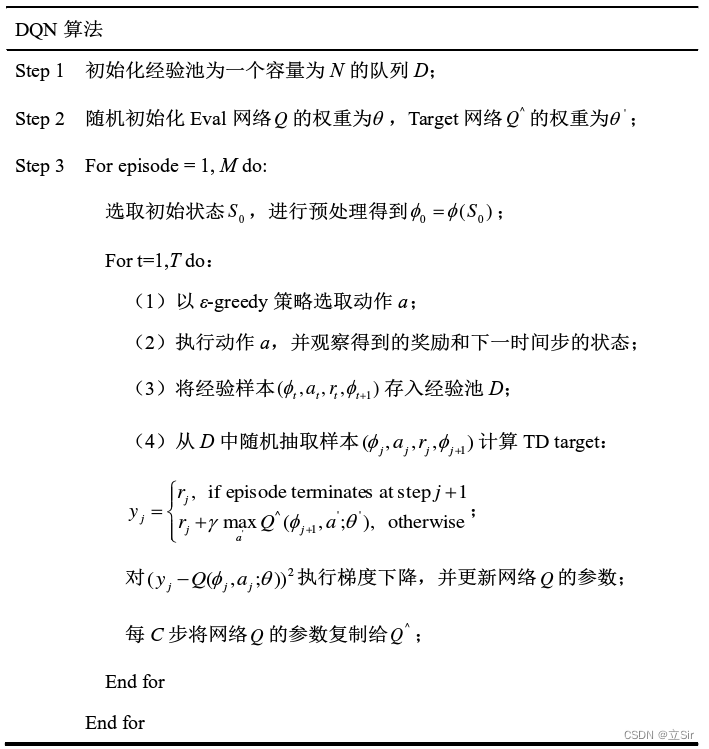
\includegraphics[width=0.8\linewidth]{pic/DQN-code.png}
    \caption{\zihao{-5} DQN算法伪代码}
    \label{map}
\end{figure}

\subsubsection{算法代码}

\begin{enumerate}
    \item 智能体


预测的时候,采用epsilon贪心进行预测。
\begin{lstlisting}[language=Python]
    # epsilon greedy
    if not exploit_flag and np.random.rand(1) < self.epsilon:
        random_action = np.random.rand(batch, self.act_shape)
        random_action = torch.tensor(random_action, dtype=torch.float32).to(self.device)
        random_action = random_action.masked_fill(~legal_act, 0)
        act = random_action.argmax(dim=1).cpu().view(-1, 1).tolist()
    else:
        feature = [
            self.__convert_to_tensor(feature_vec),
            self.__convert_to_tensor(feature_map).view(batch, *self.obs_split[1]),
        ]
        logits, _ = model(feature, state=None)
        logits = logits.masked_fill(~legal_act, float(torch.min(logits)))
        act = logits.argmax(dim=1).cpu().view(-1, 1).tolist()
\end{lstlisting}

学习的时候和预测采用一样的模型计算q\_max,再进一步计算target\_q.
\begin{lstlisting}[language=Python]
    model = getattr(self, "model")
    model.eval()
    with torch.no_grad():
        q, h = model(_batch_feature, state=None)
        q = q.masked_fill(~_batch_obs_legal, float(torch.min(q)))
        q_max = q.max(dim=1).values.detach()

    target_q = rew + self._gamma * q_max * not_done
\end{lstlisting}

\item 模型

模型概览
\begin{figure}[H]
    \centering
    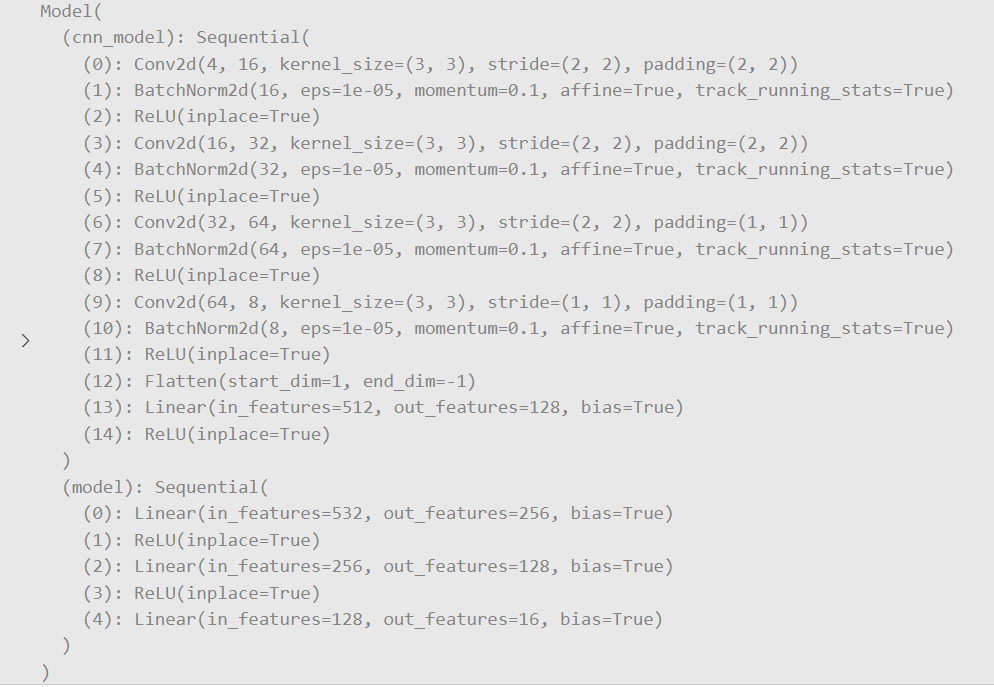
\includegraphics[width=0.8\linewidth]{pic/DQN-model.png}
    \caption{\zihao{-5} DQN算法模型}
    \label{map}
\end{figure}


前向推理

\begin{lstlisting}[language=Python]
# Forward inference
# 前向推理
def forward(self, s, state=None, info=None):
    feature_vec, feature_maps = s[0], s[1]
    feature_maps = self.cnn_model(feature_maps)

    feature_maps = feature_maps.view(feature_maps.shape[0], -1)

    concat_feature = torch.concat([feature_vec, feature_maps], dim=1)

    logits = self.model(concat_feature)
    return logits, state
\end{lstlisting}

 \item 奖励设置

为获得更高的分数,拆解出可能提高或者降低分数的动作,并设置相应的奖励及拼接权重。

\begin{lstlisting}[language=Python]
    """
    Concatenation of rewards: Here are 10 rewards provided,
    students can concatenate as needed, and can also add new rewards themselves
    奖励的拼接: 这里提供了10个奖励, 同学们按需自行拼接, 也可以自行添加新的奖励
    """
    REWARD_CONFIG = {
        "reward_end_dist": "0.1",
        "reward_win": "0.2",
        "reward_buff_dist": "0.001",
        "reward_buff": "0.001",
        "reward_treasure_dists": "0.1",
        "reward_treasure": "0.15",
        "reward_flicker": "0.1",
        "reward_step": "-0.01",
        "reward_bump": "-0.005",
        "reward_memory": "-0.005",
    }

    reward = [
        reward_end_dist * float(REWARD_CONFIG["reward_end_dist"]),
        reward_win * float(REWARD_CONFIG["reward_win"]),
        reward_buff_dist * float(REWARD_CONFIG["reward_buff_dist"]),
        reward_buff * float(REWARD_CONFIG["reward_buff"]),
        reward_treasure_dist * float(REWARD_CONFIG["reward_treasure_dists"]),
        reward_treasure * float(REWARD_CONFIG["reward_treasure"]),
        reward_flicker * float(REWARD_CONFIG["reward_flicker"]),
        reward_step * float(REWARD_CONFIG["reward_step"]),
        reward_bump * float(REWARD_CONFIG["reward_bump"]),
        reward_memory * float(REWARD_CONFIG["reward_memory"]),
    ]
\end{lstlisting}

\end{enumerate}


\subsection{Target-DQN}
\begin{figure}[H]
    \centering
    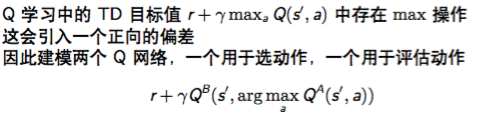
\includegraphics[width=0.8\linewidth]{pic/Double-DQN.png}
    \caption{\zihao{-5} Double-DQN}
    \label{map}
\end{figure}


\subsubsection{算法代码}

\begin{enumerate}
    
\item 智能体

预测的时候,采用epsilon贪心进行预测。这和DQN是一样的。

\begin{lstlisting}[language=Python]
    # epsilon greedy
    if not exploit_flag and np.random.rand(1) < self.epsilon:
        random_action = np.random.rand(batch, self.act_shape)
        random_action = torch.tensor(random_action, dtype=torch.float32).to(self.device)
        random_action = random_action.masked_fill(~legal_act, 0)
        act = random_action.argmax(dim=1).cpu().view(-1, 1).tolist()
    else:
        feature = [
            self.__convert_to_tensor(feature_vec),
            self.__convert_to_tensor(feature_map).view(batch, *self.obs_split[1]),
        ]
        logits, _ = model(feature, state=None)
        logits = logits.masked_fill(~legal_act, float(torch.min(logits)))
        act = logits.argmax(dim=1).cpu().view(-1, 1).tolist()
\end{lstlisting}

学习的时候和预测采用target模型来计算计算q\_max,再进一步计算target\_q.并按照指定步数更新target模型的参数。(和DQN的不同点)
\begin{lstlisting}[language=Python]

    model = getattr(self, "target_model")
    model.eval()
    with torch.no_grad():
        q, h = model(_batch_feature, state=None)
        q = q.masked_fill(~_batch_obs_legal, float(torch.min(q)))
        q_max = q.max(dim=1).values.detach()

    target_q = rew + self._gamma * q_max * not_done
\end{lstlisting}

\begin{lstlisting}[language=Python]

    # Update the target network
    # 更新target网络
    # 按照指定步数更新
    if self.train_step % self.target_update_freq == 0:
        self.update_target_q()
\end{lstlisting}

\item 模型


\begin{figure}[H]
    \centering
    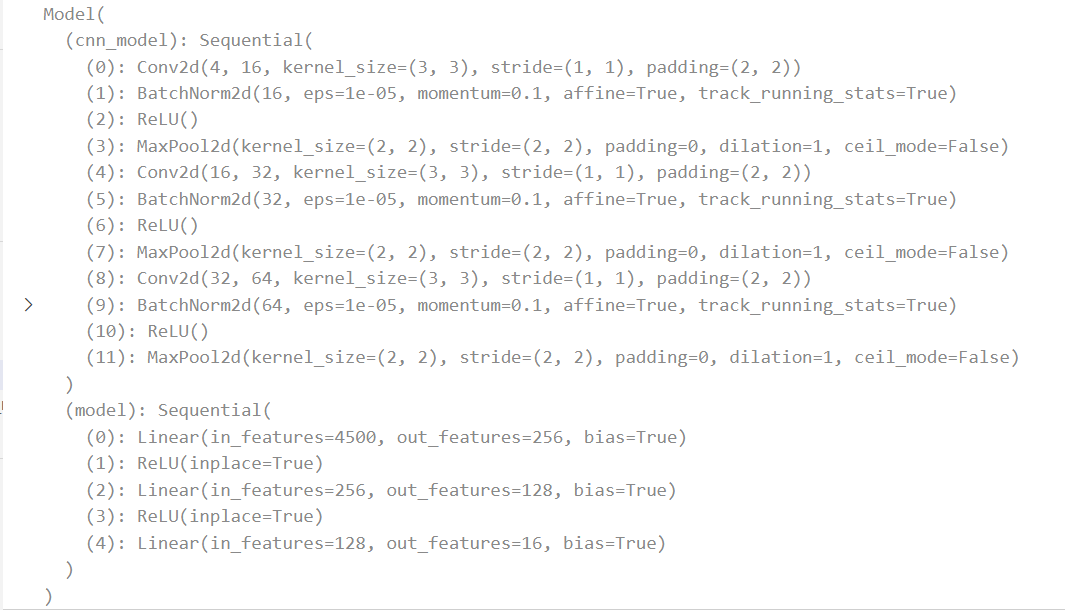
\includegraphics[width=0.8\linewidth]{pic/target-DQN-model.png}
    \caption{\zihao{-5} target-DQN算法模型}
    \label{map}
\end{figure}


\item 前向推理

\begin{lstlisting}[language=Python]
    # Forward inference
    # 前向推理
    def forward(self, s, state=None, info=None):
        feature_vec, feature_maps = s[0], s[1]
        feature_maps = self.cnn_model(feature_maps)

        feature_maps = feature_maps.view(feature_maps.shape[0], -1)

        concat_feature = torch.concat([feature_vec, feature_maps], dim=1)

        logits = self.model(concat_feature)
        return logits, state
\end{lstlisting}

\item 奖励设置

为获得更高的分数,拆解出可能提高或者降低分数的动作,并设置相应的奖励及拼接权重。

\begin{lstlisting}[language=Python]
    """
    Concatenation of rewards: Here are 10 rewards provided,
    students can concatenate as needed, and can also add new rewards themselves
    奖励的拼接: 这里提供了10个奖励, 同学们按需自行拼接, 也可以自行添加新的奖励
    """
    REWARD_CONFIG = {
        "reward_end_dist": "0.1",
        "reward_win": "0.2",
        "reward_buff_dist": "0.001",
        "reward_buff": "0.001",
        "reward_treasure_dists": "0.1",
        "reward_treasure": "0.15",
        "reward_flicker": "0.1",
        "reward_step": "-0.01",
        "reward_bump": "-0.005",
        "reward_memory": "-0.005",
    }

    reward = [
        reward_end_dist * float(REWARD_CONFIG["reward_end_dist"]),
        reward_win * float(REWARD_CONFIG["reward_win"]),
        reward_buff_dist * float(REWARD_CONFIG["reward_buff_dist"]),
        reward_buff * float(REWARD_CONFIG["reward_buff"]),
        reward_treasure_dist * float(REWARD_CONFIG["reward_treasure_dists"]),
        reward_treasure * float(REWARD_CONFIG["reward_treasure"]),
        reward_flicker * float(REWARD_CONFIG["reward_flicker"]),
        reward_step * float(REWARD_CONFIG["reward_step"]),
        reward_bump * float(REWARD_CONFIG["reward_bump"]),
        reward_memory * float(REWARD_CONFIG["reward_memory"]),
    ]
\end{lstlisting}


\end{enumerate}



\subsection{DIY}

\begin{enumerate}
\item DIY1: 修改模型

\begin{lstlisting}[language=Python]
# 前向推理
def forward(self, s, state=None, info=None):
    feature_vec, feature_maps = s[0], s[1]
    feature_maps = self.cnn_model(feature_maps)

    feature_maps = feature_maps.view(feature_maps.shape[0], -1)

    concat_feature = torch.concat([feature_vec, feature_maps], dim=1)

    logits = self.model(concat_feature)

    A = self.fc_layer3_a(logits)
    V = self.fc_layer3_v(logits)
    Q = V + A - A.mean(1).view(-1, 1)  # Q值由V值和A值计算得到

    return Q, state
\end{lstlisting}


\item DIY2: 修改学习函数

\begin{lstlisting}[language=Python]
 
    target_model = getattr(self, "target_model")
    target_model.eval()

    model = getattr(self, "model")
    model.eval()

    with torch.no_grad():
        q, h = model(_batch_feature, state=None)
        max_action = q.max(1)[1].view(-1, 1)
        next_q, next_h = target_model(_batch_feature, state=None)
        next_q = next_q.masked_fill(~_batch_obs_legal, float(torch.min(next_q)))
        q_max = next_q.gather(1, max_action).detach().flatten()
\end{lstlisting}

\end{enumerate}
\section{实验记录及结果展示}

\subsection{实验记录}
主要是通过调整奖励、学习率、模型以及Q值计算公式等来获得更高的参数。
\begin{figure}[H]
    \centering
    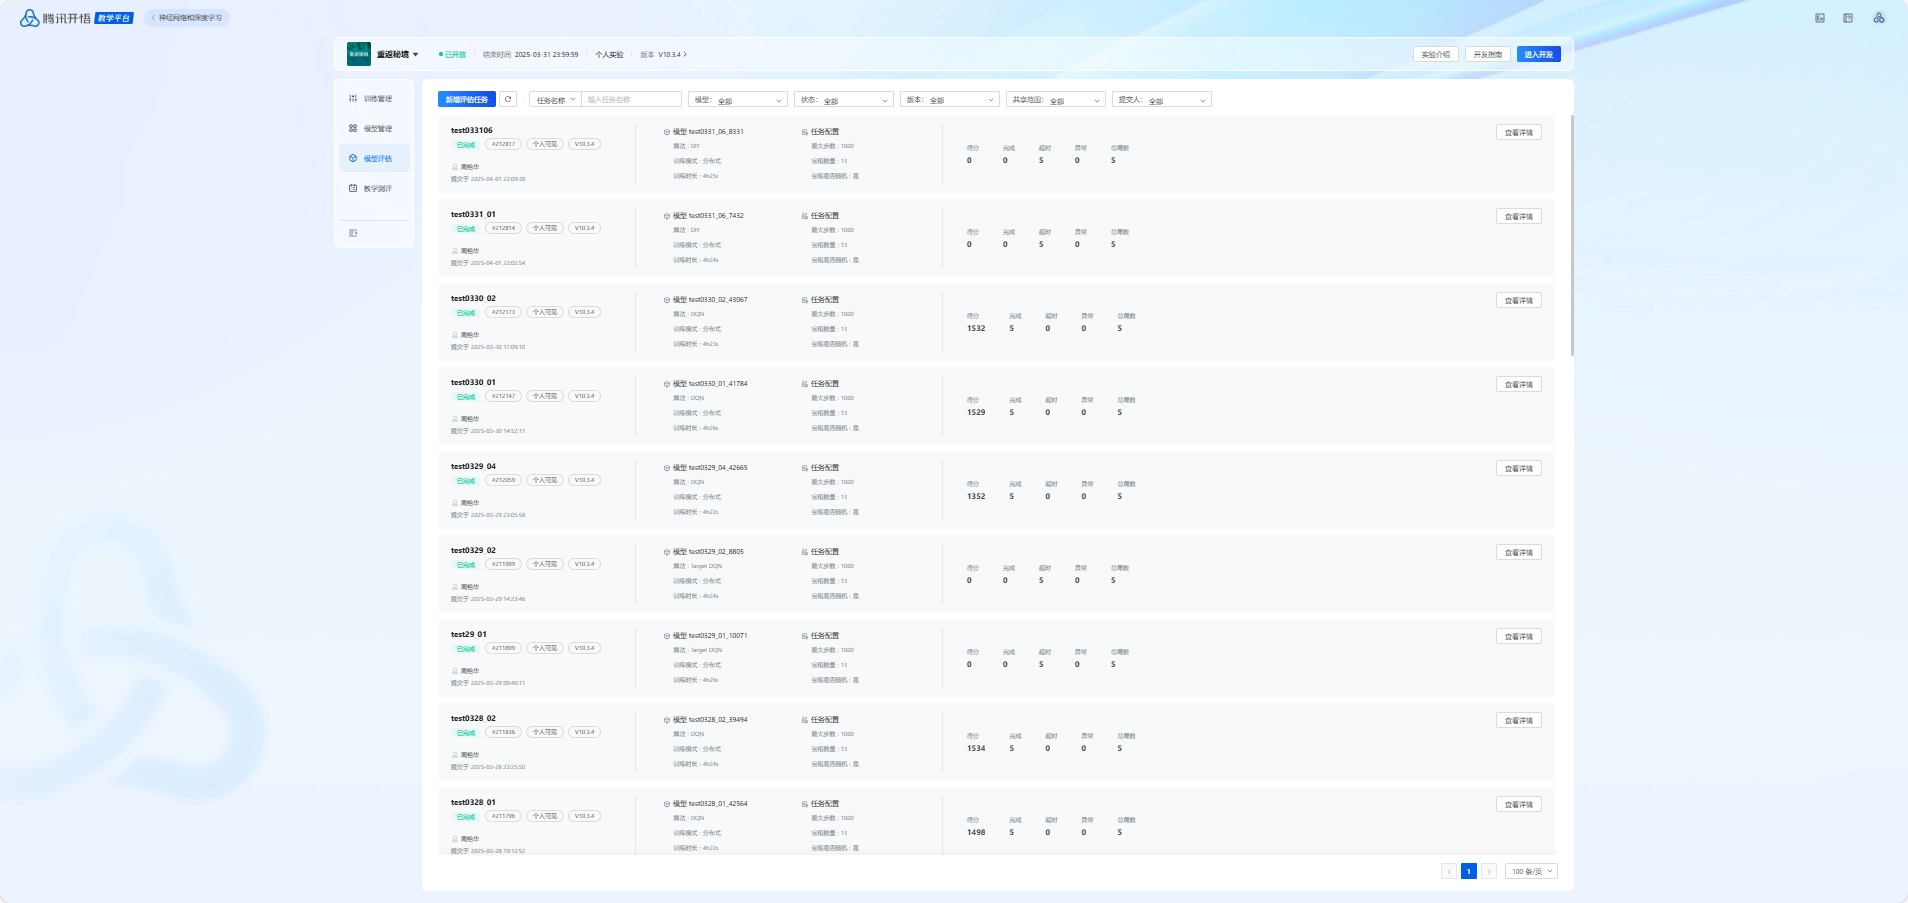
\includegraphics[width=0.8\linewidth]{pic/record-1.png}
    \caption{\zihao{-5} 实验记录1}
    \label{map}
\end{figure}

\begin{figure}[H]
    \centering
    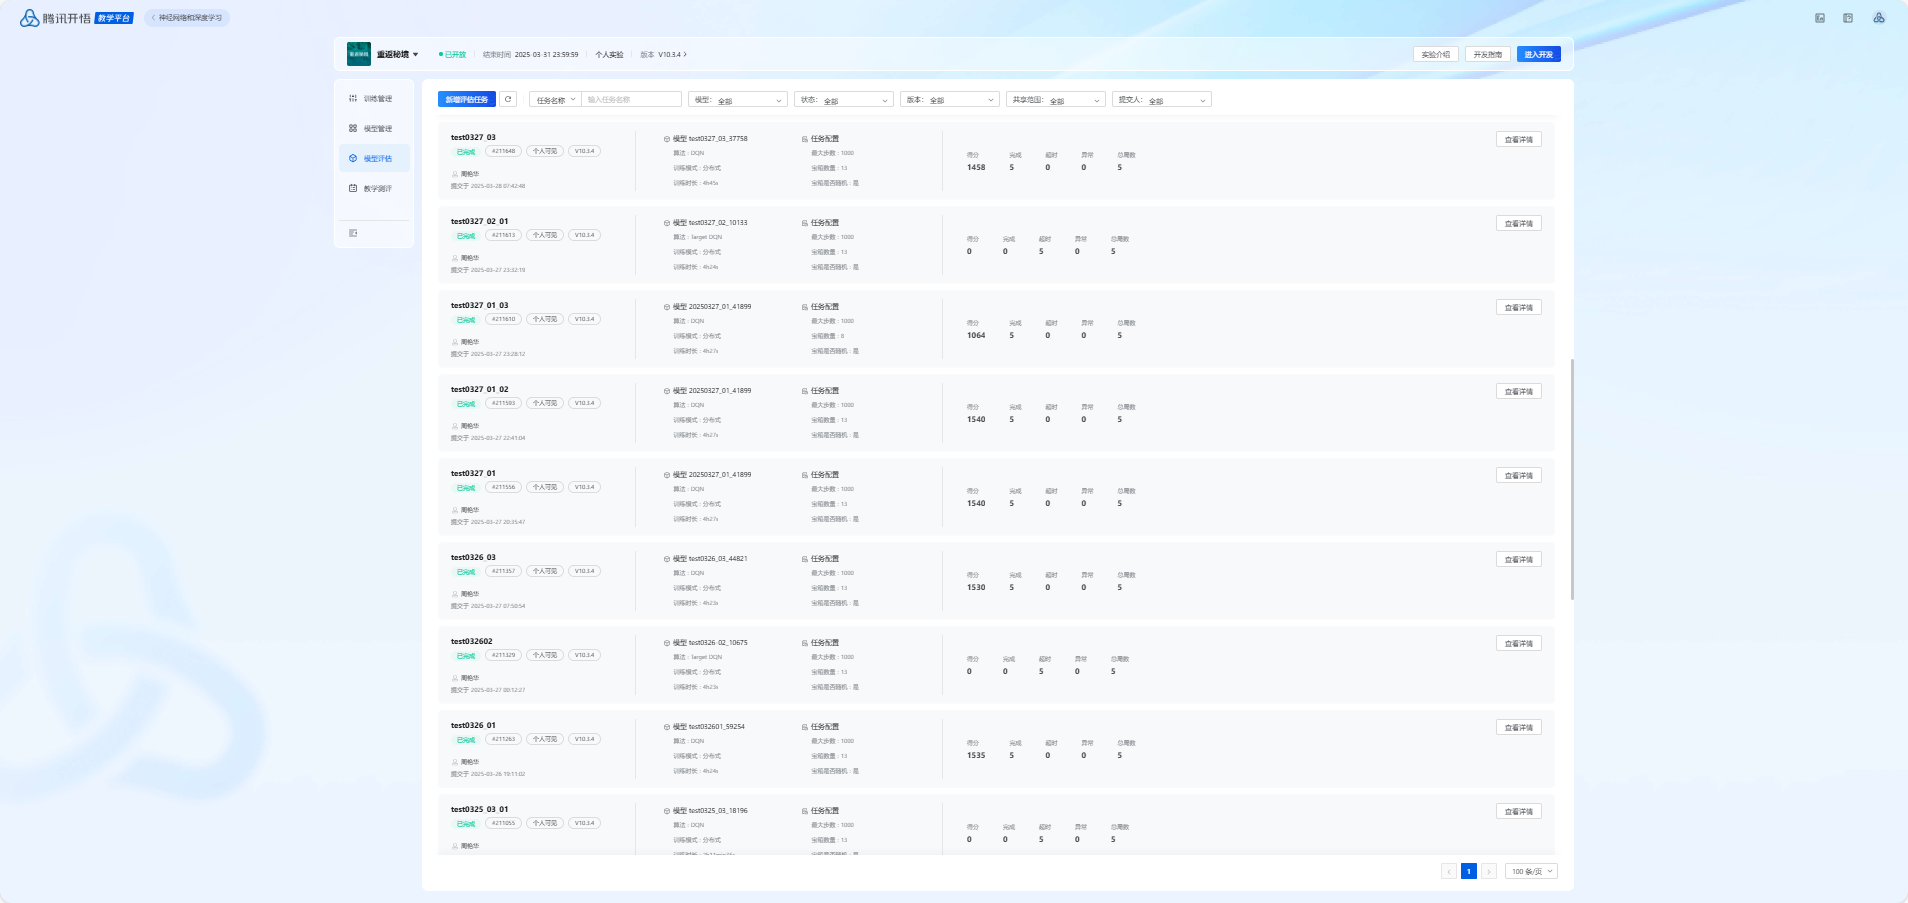
\includegraphics[width=0.8\linewidth]{pic/record-2.png}
    \caption{\zihao{-5} 实验记录2}
    \label{map}
\end{figure}

\begin{figure}[H]
    \centering
    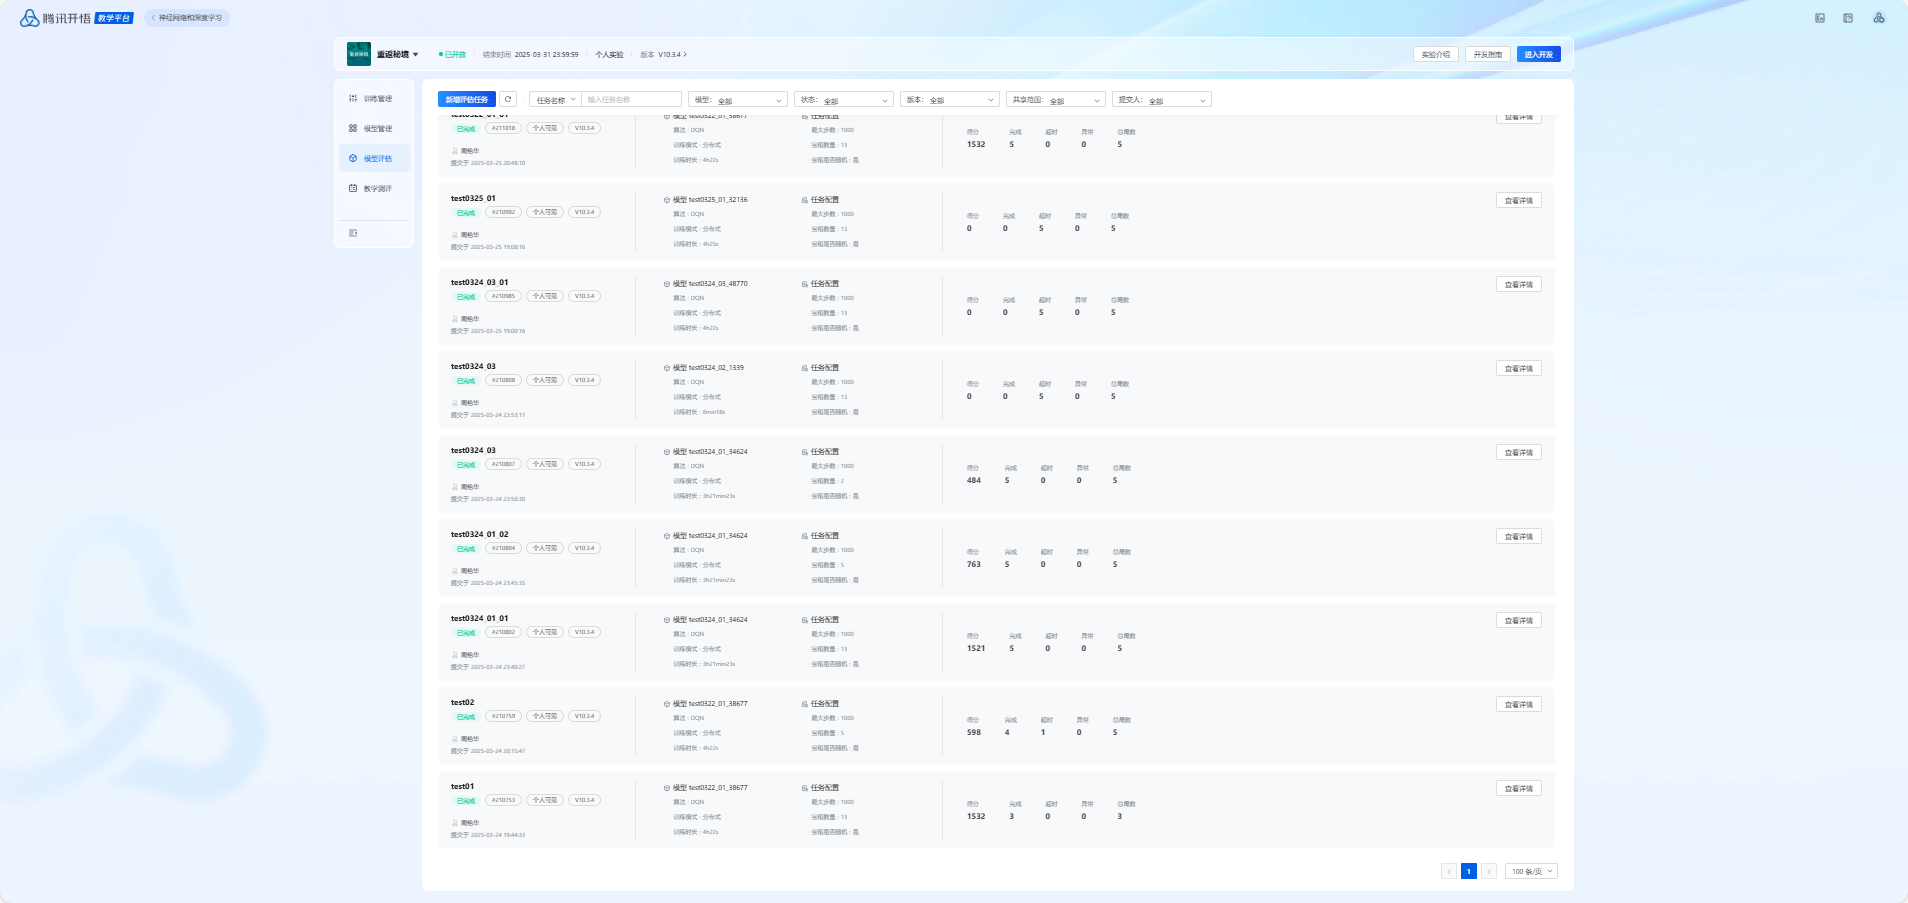
\includegraphics[width=0.8\linewidth]{pic/record-3.png}
    \caption{\zihao{-5} 实验记录3}
    \label{map}
\end{figure}



\subsection{最佳分数}
多次实验得到的模型,在最大步数1000,宝箱数量13个的情况下,使用DNQ算法得到的最佳分数为1400.
\begin{figure}[H]
    \centering
    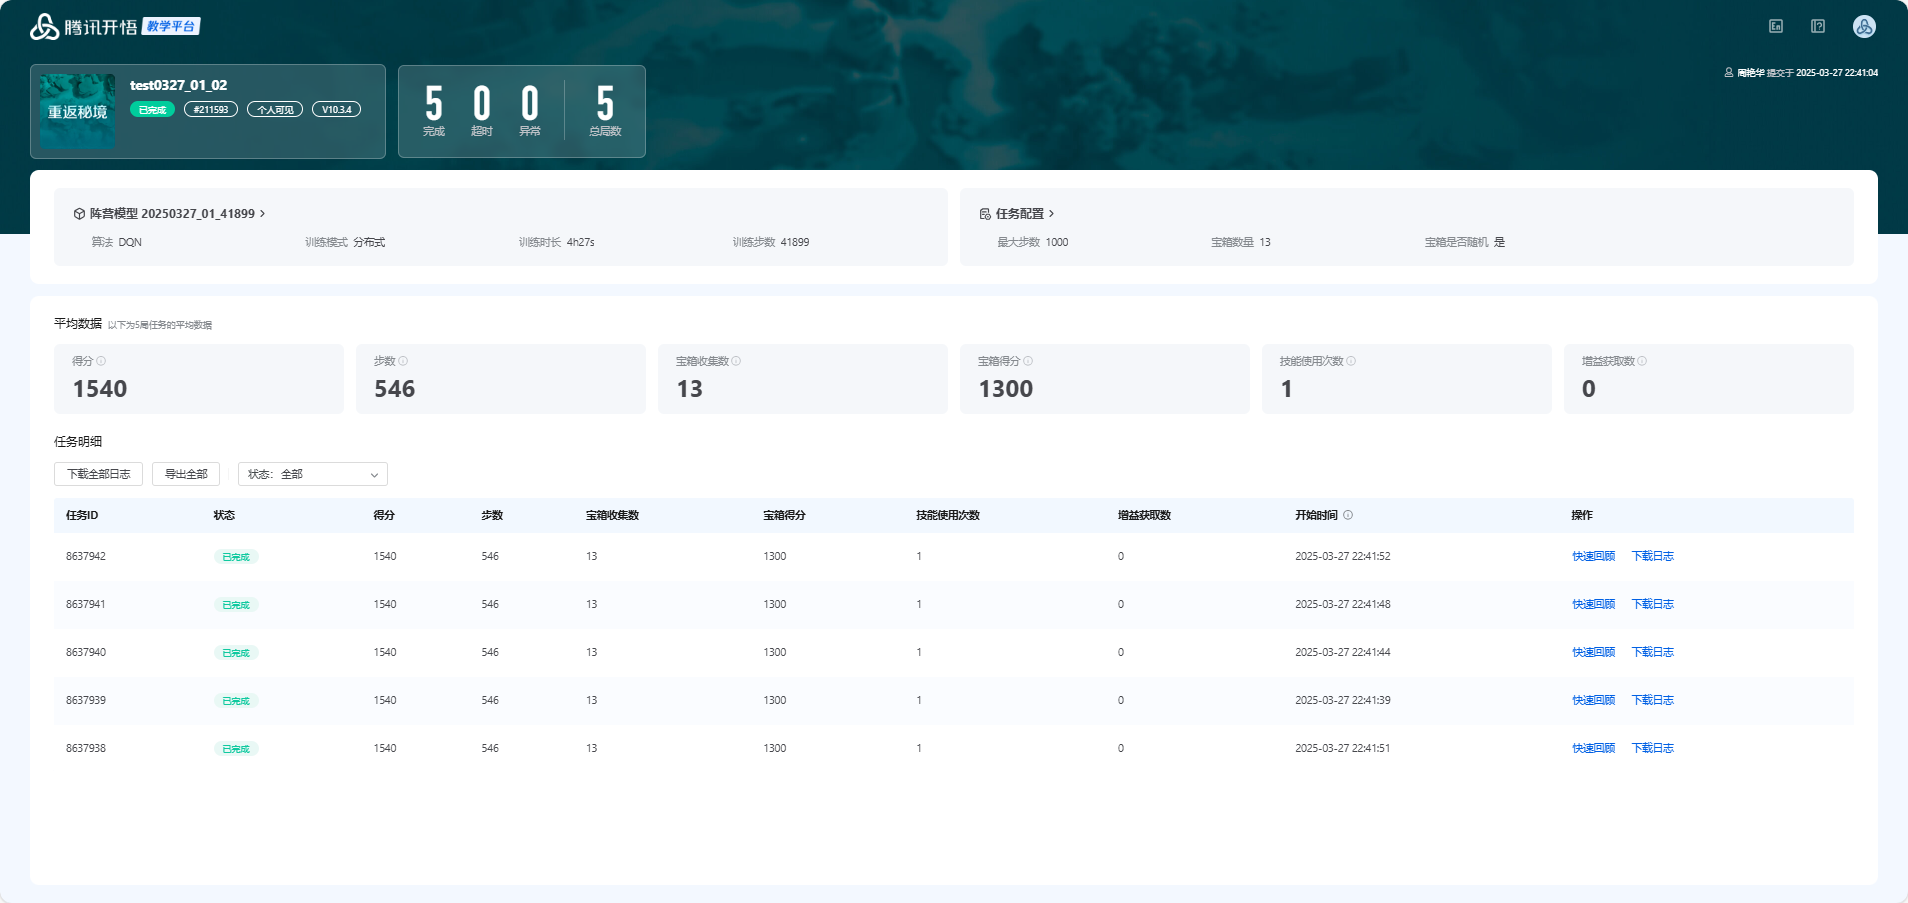
\includegraphics[width=0.8\linewidth]{pic/best-score.png}
    \caption{\zihao{-5} 最佳分数}
    \label{map}
\end{figure}
下图是最佳分数对应的路径概览。可以看出,如果能捡到加速,分数有可能能更高。(不过试了几次没有找到更高的)
\begin{figure}[H]
    \centering
    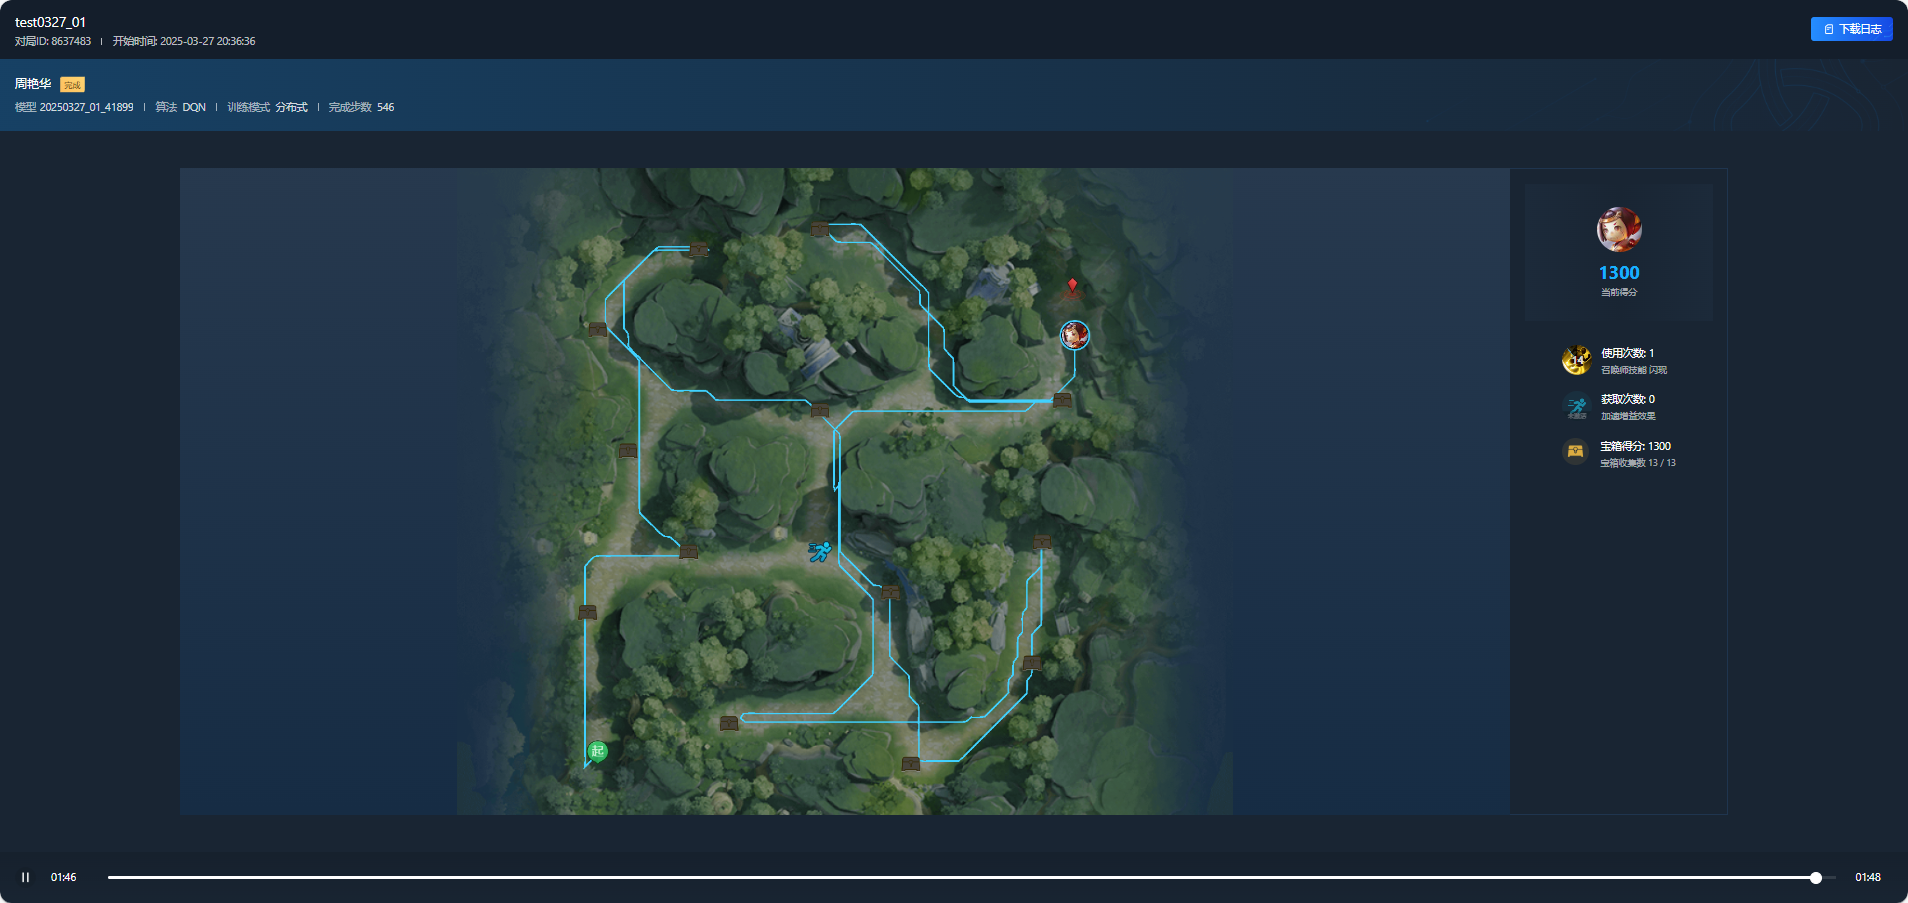
\includegraphics[width=0.8\linewidth]{pic/best-map.png}
    \caption{\zihao{-5} 路径概览}
    \label{map}
\end{figure}

\end{document}
